%!TEX root = ../diplom.tex
\newcommand{\tK}{\widetilde K}
\section{Численное моделирование морского волнения}

Для выполнения вычислений в режиме реального времени применяются
мощные компьютеры. Это позволяет прогнозировать развитие морского волнения и
результаты активно используют океанологи и метеорологи. Однако за это
приходится «платить» низким пространственным разрешением, упрощением исходных
уравнений и моделированием только длинно-волновой составляющей спектра
волнения.  Для оценки эффективности работы радиолокационной аппаратуры больше
подходит хорошо известный подход, опирающийся на модель спектра волнения. В
этом случае морская поверхность представляется в виде набора синусоид
(гармоник), амплитуда которых вычисляется по спектру
волнения \cite{longe-higgins}, \cite{karaev}. При
таком подходе смоделированная морская поверхность утрачивает ряд свойств,
присущих реальной морской поверхности, но становится более удобной для счета и
моделирование может быть проведено на домашнем компьютере. Именно
этот подход выбран для моделирования морской поверхности в данном исследовании.
Надо отметить, что для выбранного подхода качество моделирования зависит от
используемого спектра волнения и от численной реализации процедуры
моделирования.

Предполагается, что гармоники не взаимодействуют друг с другом, поэтому возвышения поверхности, орбитальные
скорости, уклоны и другие характеристики волнения являются суммой
независимых гармоник.

\subsection{Общие сведения}%
\label{sec:obshchie_poniatiia}
Определим ряд общих понятий, описывающих возвышение взволнованной морской поверхности в рамках теории случайных пространственно-временных полей. В этом случае поверхность представляется в виде суммы синусоидальных волн со случайными фазами 
\begin{equation}
    \label{eq:surface}
    \xi(\vec r,t) = \sum\limits_{n=-\infty}^{\infty} 
        A_n(\vec \kappa_n) e^{i(\omega_n t + \vec \kappa_n \vec r + \psi_n)},
\end{equation}
где $\psi_n$ -- случайная фаза,
равномерно распределенная в интервале от $0$ до  $2 \pi$, 
$A_n (\vec \kappa_n)$ -- комплексная амплитуда гармоники с волновым числом
$\vec \kappa_n$ и временной частотой  $\omega_n$, связанной с  $\vec \kappa_n$ известным
дисперсионным соотношением
\begin{equation}
    \omega(\kappa) = \sqrt{\kappa g + \alpha \kappa^3},
\end{equation}
где $g$ -- ускорение свободного падения,  $\alpha$ -- коэффициент, 
зависящий от свойств жидкости.


Корреляционную функцию $K_{\xi}(\vec r,t)$ поля  $\xi(\vec r, t) $ определим
стандартным образом \cite{tihonov}
 \begin{equation}
    \label{eq:corr}
    K_{\xi}\qty[\vec r_1, \vec r_2, t_1,t_2] = \mean{\xi(\vec r_1,t_1)\xi^*(\vec r_2,t_2)}
\end{equation}

Поле высот в нашей задаче считаем стационарным в широком смысле, то есть 
$K_{\xi}\qty[\vec r_{1},\vec r_{2},t_{1},t_{2}] = K_{\xi}\qty[\vec \rho = \vec
r_{2} - \vec r_1, \tau=t_{2}-t_{1}]$. Будем считать, гармоники
независимыми друг от друга, а значит перекрестные члены в уравнении
\eqref{eq:corr} равны нулю.

Тогда корреляционная функция поверхности
\eqref{eq:surface} примет следующий вид
\begin{equation}
    \label{eq:surface_corr}
    K_{\xi}\qty[\vec \rho,\tau] = \sum\limits_{n=-\infty}^{\infty} 
    \frac{A_n^2}{2} 
    \exp{i \qty(\vec \kappa_n \vec \rho + \omega \tau)}
\end{equation}

Для решения задачи моделирования отраженного от морской поверхности импульса
достаточно рассматривать мгновенный снимок моделируемой поверхности, в момент
отражения
а значит можно положить $\tau = \const = 0$  и  тогда $K_\xi[\rho,\tau] = K_\xi [\rho]$.

В этом случае справедлива формула Винера-Хинчина \cite{tihonov}
\begin{equation}
    \begin{gathered}
    \label{eq:Viner-Hinchin}
        S_\xi(\vec k) \int\limits_{-\infty}^{\infty} K_\xi \qty[\vec \rho] \exp{- i
        \vec \kappa \vec \rho} \dd \rho \\
        K_\xi[\rho] = \frac{1}{2 \pi} \int\limits_{-\infty}^{\infty} S_\xi (\vec k) \exp{+ i
        \vec \kappa \vec \rho} \dd \rho. 
    \end{gathered}
\end{equation}


Предположим, что спектр морского волнения можно представить в виде функции с
разделяющимися переменными, где $S_{\xi}(\kappa)$ определяет зависимость
спектральной плотности мощности от волнового числа, а функция $\Phi(\kappa, \phi)$ -- 
описывает зависимость спектральной плотности мощности от азимутального угла для
выбранного волнового числа
\begin{equation}
    S_\xi(\vec \kappa) = S_\xi(\kappa) \Phi_\xi(\kappa, \phi),
\end{equation}
где $\kappa = \sqrt{\kappa_x^2 + \kappa_y^2}$,  $\phi = \arctg
\frac{\kappa_x}{\kappa_y}$. Для
удобства, угловое распределение нормируется так, чтобы
\begin{equation}
\int\limits_{-\infty}^{\infty} \Phi_\xi(\kappa,\phi) \dd \phi = 1.
\end{equation}

\subsection{Двумерная модель поверхностного волнения}%
\label{sec:dvumernaia_model_poverkhnostnogo_volneniia}

В соответствии с предыдущим разделом, для моделирования случайной поверхности
$\xi(\vec r,t)$ будем использовать её представление в виде суперпозиции
плоских волн с различными частотами и случайными фазами $\psi_{nm}$, бегущих
под разными азимутальными углами $\phi_m$ \cite{karaev}:
\begin{figure}[H]
    \centering
    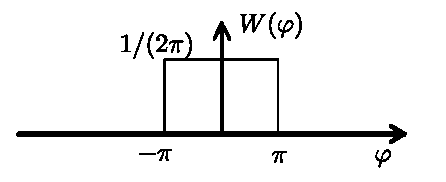
\includegraphics[scale=1]{fig/image65}
    \caption{Плотность вероятности случайной фазы $\phi$.}
    \label{fig:phase}
\end{figure}

\begin{equation}
    \label{eq:surface2d}
    \xi(\vec r,t) = \sum\limits_{n=1}^{N} \sum\limits_{m=1}^{M}
    A_n(\kappa_n) \cdot
    F_m(\kappa_n,\phi_m) \cos \qty(\omega_n t + \vec \kappa \vec r + \psi_{nm}),
\end{equation}
где $\psi_{nm}$ -- случайная фаза, равномерно распределенная в интервале от $0$
до $2 \pi$ (см. рис. \ref{fig:phase}), $F_m(\kappa_n, \phi_m)$ -- азимутальное
распределение для гармоники с волновым числом  $\kappa_n$,  $\vec \kappa_n =
(\kappa_{nx}, \kappa_{ny})$ -- 
волновой вектор. 
%В соответствии с
%центральной предельной теоремой \cite{tihonov}. 

Амплитуда $n$-ой гармоники $A_n$ есть
мощность на интервале $\Delta \kappa_n$, которая вычисляется по спектру моделируемой
поверхности $S_\xi(\kappa)$. Пользуясь определением корреляционной
функции \eqref{eq:surface_corr} и формулой Винера-Хинчина
\eqref{eq:Viner-Hinchin} получим точное выражение для нахождения амплитуды
$n$-ой гармоники  $A_n$

\begin{gather}
    K_{\xi}[\vec \rho, \tau] = \frac{1}{(2 \pi)^2}  \int\limits_{-\infty}^{\infty}  S_{\xi}(\vec \kappa) e^{i \vec \kappa \vec \rho} \dd \vec k = 
    \frac{1}{(2 \pi)^2} 
        \int\limits_{-\infty}^{\infty}
        \int\limits_{- \pi}^{\pi} 
    S_\xi(\kappa) \Phi_\xi(\phi) \kappa e^{i \vec \kappa\vec \rho} \dd \kappa \dd \phi = \\
    = \frac{1}{(2 \pi)^2} \int\limits_{-\infty}^{\infty} \kappa S_\xi
    (\kappa) e^{i \vec \kappa 
    \vec \rho} \dd \kappa = \sum\limits_{n=-\infty}^{\infty} \frac{(A_n(\vec
\kappa_n))^2}{2} e^{i \vec \kappa_n \vec \rho} 
\end{gather}

\begin{equation}
    \label{eq:Amplitude}
    A_n(\kappa_n) = \frac{1}{2 \pi} \sqrt{\int\limits_{\Delta \kappa_n} 2
        \kappa S_\xi(\kappa)
    \dd \kappa}
\end{equation}

%При достаточно большом $n \to \infty$ ($\Delta \kappa_n \to 0$) можно интегрировать
%прямоугольником
%\begin{equation}
    %A_n(\kappa_n) = \frac{1}{2 \pi} \sqrt{ 2 \kappa S_\xi(\kappa_n) \Delta
    %\kappa_n}
%\end{equation}
%c погрешностью, пропорциональной $\Delta A_n \sim  \sqrt{\frac{\dd \kappa
    %S_\xi(\kappa)}{\dd \kappa}
%\Delta \kappa_n^2}$. 

Для удобства, введем новое обозначение для спектра
$S(\kappa_n)\equiv \kappa_n S_\xi (\kappa_n)$.

Аналогично вычислению амплитуд, можно вычислить азимутальное распределение $F_m$  следующим образом:
\begin{equation}
    F_{nm}(\kappa_n,\phi_m) = \sqrt{\int\limits_{\Delta \phi_m}
    \Phi_{\xi}(\kappa_n,\phi) \dd \phi},
\end{equation}
где $\Delta \phi = \frac{2\pi}{M}$ -- шаг по азимутальному углу.

\begin{figure}[ht]
    \def\spec{fig/water/spectrum}
    \begin{subfigure}{0.5\linewidth}
        \centering
        \includegraphics[scale=1,page=1]{\spec}
        \caption{}
    \end{subfigure}
    \begin{subfigure}{0.5\linewidth}
        \centering
        \includegraphics[scale=1,page=2]{\spec}
        \caption{}
    \end{subfigure}
    \caption{Спектр высот $S(\kappa)$ для разных скоростей ветра: синяя кривая
    - 5 м/с, красная кривая - 10 м/с, коричневая кривая - 15 м/с, (a)
Ku-диапазон, (b) C-диапазон.}
    \label{fig:spectrum_heights}
\end{figure}

\begin{figure}[ht]
    \def\angdistrib{fig/water/angles_distribution}
    \begin{subfigure}{0.5\linewidth}
        \centering
        \includegraphics[scale=1,page=1]{\angdistrib}
        \caption{}
    \end{subfigure}
    \begin{subfigure}{0.5\linewidth}
        \centering
        \includegraphics[scale=1,page=2]{\angdistrib}
        \caption{}
    \end{subfigure}
    \caption{Спектр $\Phi(\kappa, \phi)$ для разных соотношений  $\kappa /
    \kappa_m$}
    \label{fig:angles_distrib}
\end{figure}


Графики $S(\kappa)$ и  $\Phi_\xi(\kappa)$ для приведены на рис.
\ref{fig:spectrum_heights} и рис. \ref{fig:angles_distrib} соответственно
\cite{ryabkova}. 
Вычисления на рис. \ref{fig:spectrum_heights} выполнены для скоростей ветра 
$U_{10} = 5$ м/с (синяя кривая), 10 м/с (красная кривая) и 15 м/с (коричневая
кривая), также на  рис. \ref{fig:spectrum_heights} учитывается граничное волновое число
для моделирования поверхности для двух диапазонов излучения: $Ku$ и $C$. В
рамках двух масштабной модели  рассеивающей поверхности \cite{bass-and-fuks}.
Волновое число $\kappa_m$ соответствует  максимуму спектра волнения  $S(\kappa)$. Стоит
заметить, что с ростом скорости ветра число используемых гармоник, необходимых
для получения одинакового качества моделирования,
возрастает. 

Это обусловлено тем, что растет интервал волновых чисел $\kappa$, на котором
определен спектр волнения. 

На рис. \ref{fig:water} изображены поверхности,
На рис. \ref{fig:water_photo} представлена фотография взволнованной морской
поверхности для сравнения с рис. \ref{fig:water},
построенные по формуле \eqref{eq:surface2d}.

Для рис. \ref{fig:water}a доминантная длина волны равна 23 м, высота
значительного волнения 0.83 м, для рис. \ref{fig:water}b доминантная длина
волны равна 206 м, а высота значительного волнения 6.58 м.

\begin{figure}[h!]
    \begin{subfigure}{0.5\linewidth}
        \centering
        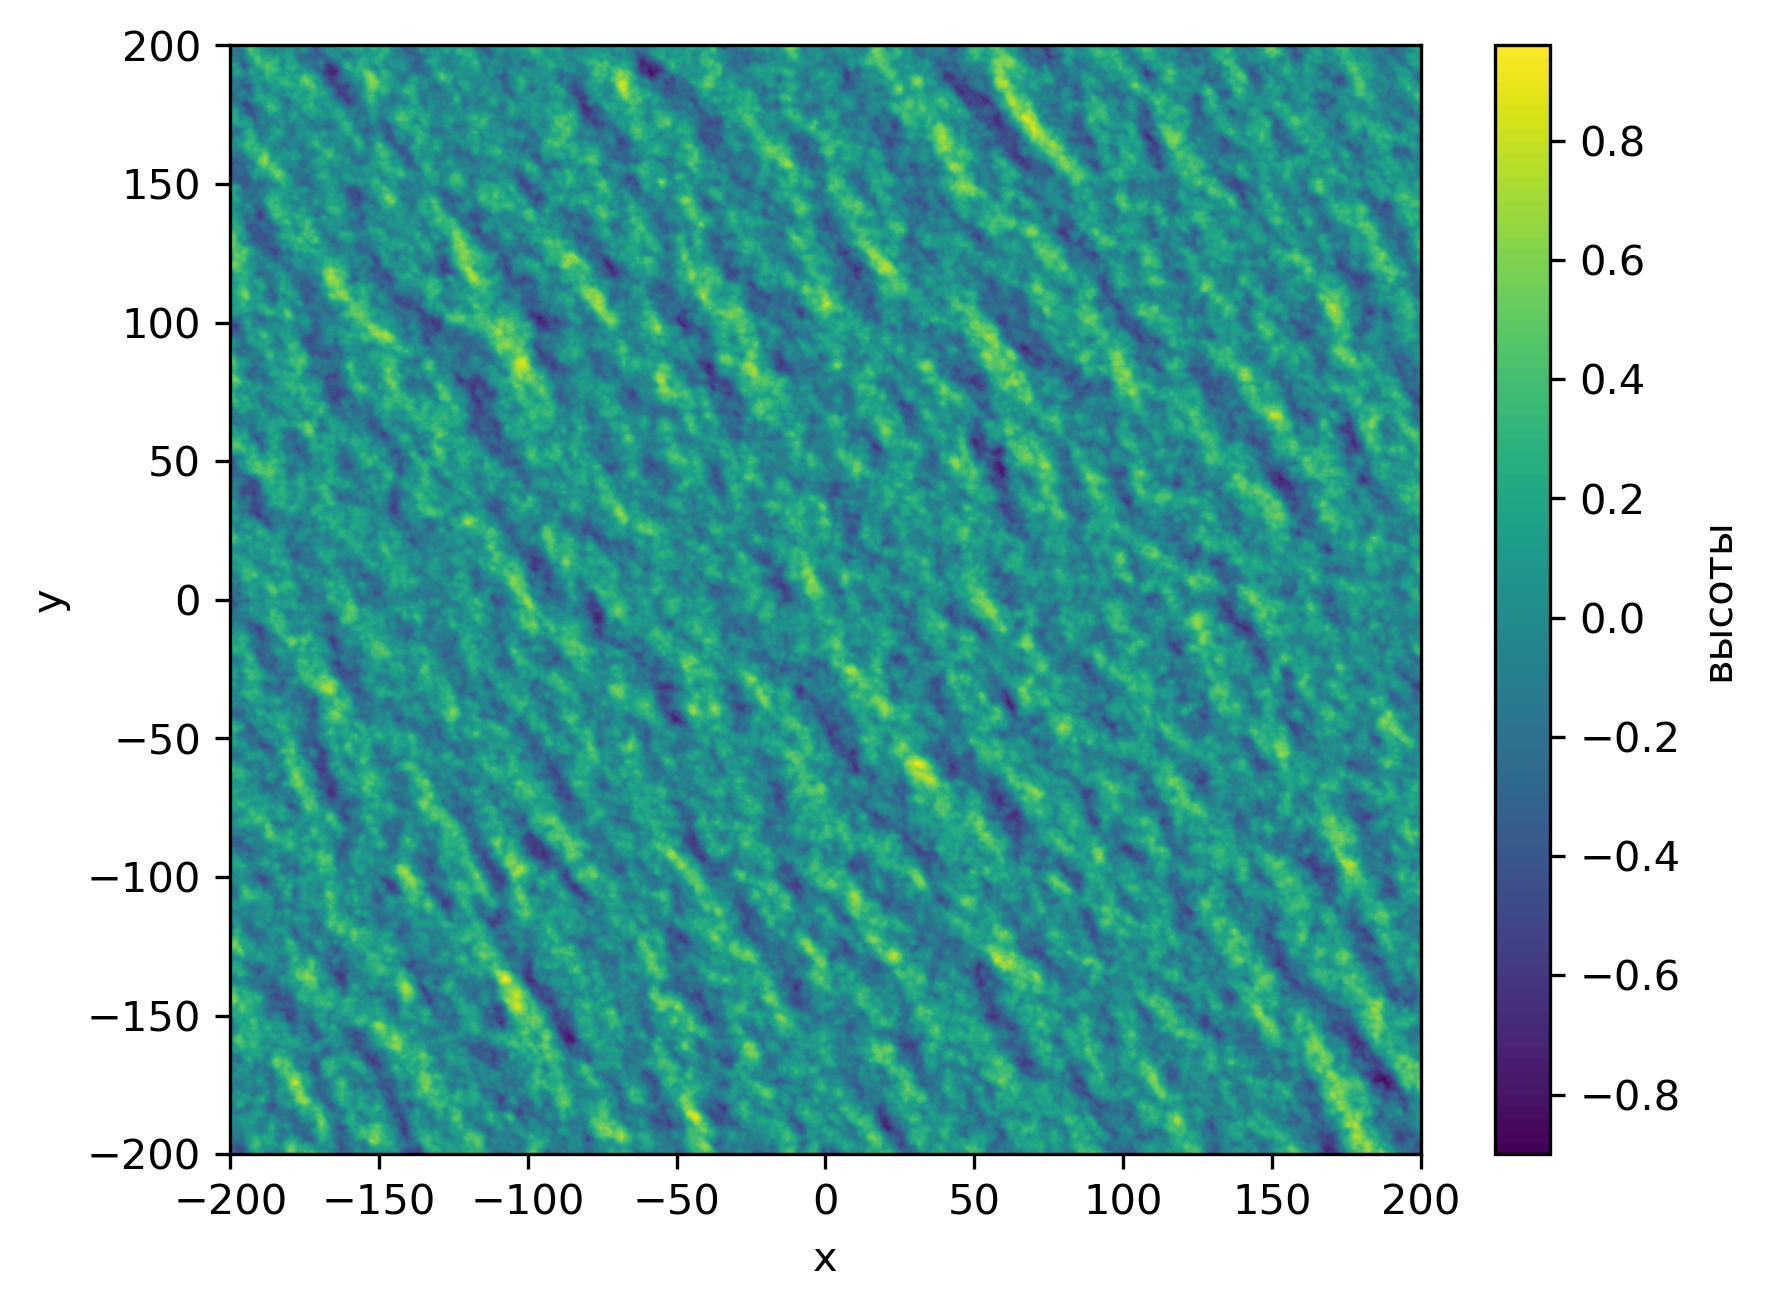
\includegraphics[width=\linewidth]{img/heights5}
        \caption{}
    \end{subfigure}
    \begin{subfigure}{0.5\linewidth}
        \centering
        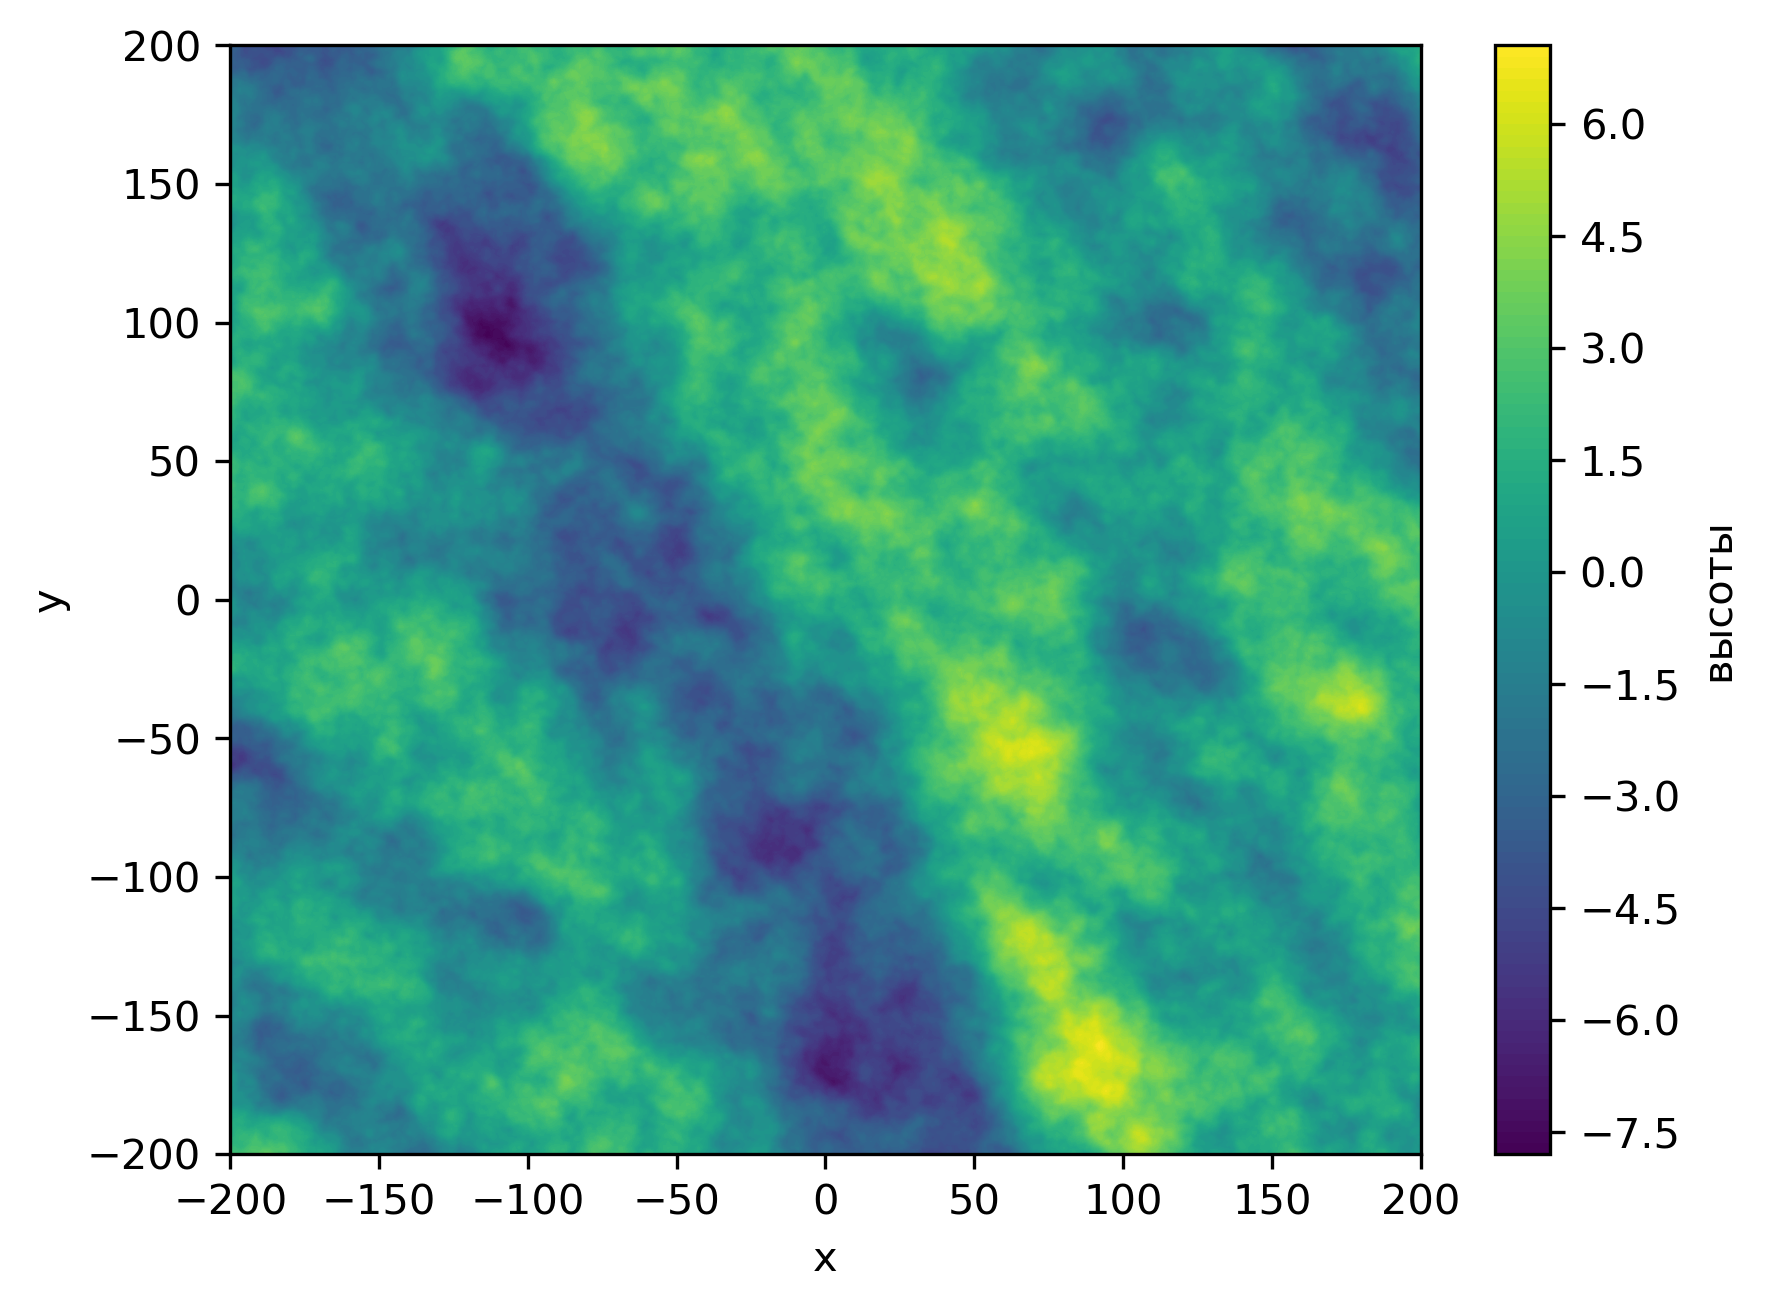
\includegraphics[width=\linewidth]{img/heights15}
        \caption{}
    \end{subfigure}
    \caption{ Полутоновое изображение смоделированного поля высот для
        направления ветра $30^\circ$ и разных скоростей ветра
        (a) $U_{10} = 5 \text{м}/\text{c}$;
        (b) $U_{10} = 15 \text{м}/\text{c}$;
}
    \label{fig:water}
\end{figure}
\begin{figure}[h!]
    \centering
    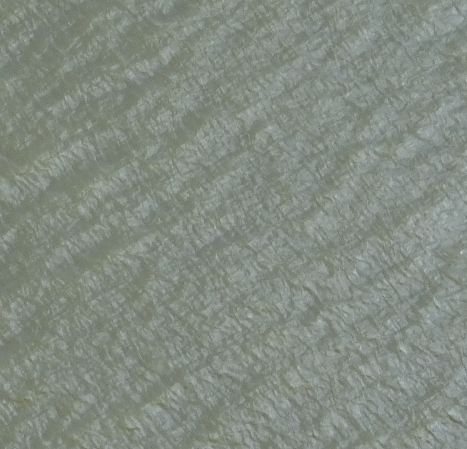
\includegraphics[width=0.49\linewidth]{img/water_photo.png}
    \caption{Фотография водной поверхности}
    \label{fig:water_photo}
\end{figure}

Такой подход к моделированию морской поверхности является одним из самых простых и достаточно эффективным, но у него есть существенные недостатки.

Прежде всего, моделируемая поверхность получается симметричной, хотя реальная поверхность асимметрична: передний склон волны более крутой и короткий по сравнению с задним склоном.

Кроме того, площадь гребней меньше площади впадин для морского волнения, что
также не находит отражения в свойствах моделируемой поверхности. Эти отличия
модельной поверхности от морской поверхности не позволят смоделировать так
называемые поправки на состояние морской поверхности \cite{fu},
\cite{pustovoytenko}. 
Правильно смоделировать именно поправки на состояние крайне важно для получения
достоверных результатов при моделировании формы импульса
отраженного радиолокационного
сигнала. Как решить эту проблему обсудим в дальнейшем.


Для моделирования морской поверхности необходимо определиться с числом
гармоник. Надо отметить, что с ростом скорости ветра число используемых
гармоник, необходимых для получения одинакового качества моделирования, будет
возрастать. Это обусловлено тем, что увеличивается интервал волновых чисел
$\kappa$, на котором определен спектр волнения (см. рис.
\ref{fig:spectrum_heights}). 

Следующая задача, которую надо решить, связана с тем, как расположить гармоники
по оси волновых чисел. Максимуму спектра волнения соответствует волновое числа
$\kappa_m$, левую границу спектра определим как $\frac{\kappa}{4}$, а правую
границу обозначим $\kappa_{cut}$. Это значение будет различаться для Ku- и
C-диапазонов. Формула для определения была получена в \cite{karaev} и приведена  
в приложении \ref{sec:code}\ref{lst:spectrum}.


Самый простой вариант расположения гармоник это равномерный шаг, который можно определить следующим образом:
\begin{equation}
    \Delta \kappa = \frac{k_{cut}}{(N-1)}, 
\end{equation}
где $\kappa_{cut}$ -- граничное волновое число, $N$ -- число грамоник.



Критерием качества моделирования, а также оптимального выбора числа гармоник
была выбрана близость следующих корреляционных функций высот:
\begin{equation}
    \begin{gathered}
        \label{eq:KK}
        K[\rho] = \int\limits_{-\infty}^{\infty} S(\kappa) \cos(\kappa\rho) \dd \kappa\\
        \tK(\rho) = \sum\limits_{n=1}^{N} \frac{A_n^2}{2} \cos(\kappa_n \rho)
    \end{gathered}
\end{equation}




Сравнение корреляционной функции $\tK[\rho]$ полученной по модели, с
теоретической корреляционной функцией $K[\rho]$   позволит оценить качество
модели.  

Если посмотреть на форму спектра, то задача усложняется тем,
что спектр высот является узким и в основном сосредоточен вблизи пика
(длинноволновой составляющей спектра волнения).  Кроме того, равномерный шаг
приводит к появлению <<артефактов>>, что хорошо видно на рис.
\ref{fig:corr_h_lin}.
Вычисления выполнены дл полностью развитого ветрового волнения и трех скоростей
ветра: 5 м/с, 10 м/с и 15 м/с. Число гармоник для всех скоростей ветра было
выбрано равным 256. Для удобства сравнения разных скоростей ветра, при
построении, корреляционные функции были нормированы на дисперсию высот.
\def\correlation{fig/water/correlation}
\begin{figure}[H]
    \centering
    \begin{subfigure}{0.49\linewidth}
        \centering
        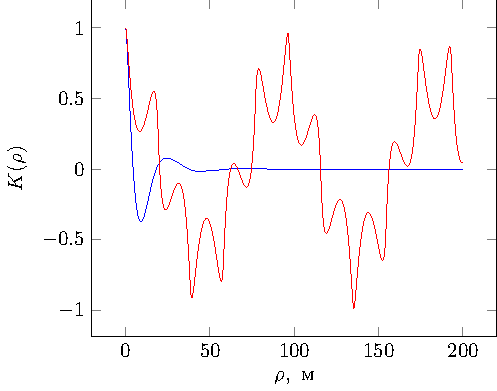
\includegraphics[scale=1,page=1]{\correlation}
    \end{subfigure}
    \hfill
    \begin{subfigure}{0.49\linewidth}
        \centering
        \includegraphics[scale=1,page=2]{\correlation}
    \end{subfigure}
    \begin{subfigure}{0.49\linewidth}
        \centering
        \includegraphics[scale=1,page=3]{\correlation}
    \end{subfigure}
    \caption{Нормированная корреляционная функция высот для равномерного распределения и 3-х
    скоростей ветра: (a) 5 м/с,  (b) 10 м/с, (c) 15 м/с и числе
гармоник $N=256$}
    \label{fig:corr_h_lin}
\end{figure}
Частично от артефактов можно избавиться, выбрав неравномерный шаг. Нужно задать
распределение таким образом, чтобы вблизи малых значений волнового числа
(вблизи пика спектра) плотность расположения гармоник была существенно выше,
чем при больших $\kappa$.

Можно предложить несколько вариантов неравномерного распределения и ниже
протестируем два варианта.

В качестве первого распределения выберем следующую формулу
\begin{equation}
    k_i = k_{min} + \frac{k_{cut} - k_{min}}{(N-1)^2} (i-1)^2
\end{equation}

Для второго распределения выберем <<логарифмический>> шаг и положения гармоник
определим следующим образом
\begin{equation}
    k_i = k_{i-1} \cdot \Delta  \kappa
\end{equation}

На рис. \ref{fig:corr_h_quad} и \ref{fig:corr_h_log} видно, что лучше всех
<<работает>> логарифмическое разбиение интервала волновых чисел.
\begin{figure}[H]
    \centering
    \begin{subfigure}{0.49\linewidth}
        \centering
        \includegraphics[scale=1,page=9]{\correlation}
    \end{subfigure}
    \hfill
    \begin{subfigure}{0.49\linewidth}
        \centering
        \includegraphics[scale=1,page=10]{\correlation}
    \end{subfigure}
    \begin{subfigure}{0.49\linewidth}
        \centering
        \includegraphics[scale=1,page=11]{\correlation}
    \end{subfigure}
    \caption{Нормированная корреляционная функция высот для логарифмического распределения и
    4-х скоростей ветра: (a) 5 м/с,  (b) 10 м/с, (c) 15 м/с и числе}
    \label{fig:corr_h_quad}
\end{figure}


\begin{figure}[ht]
    \centering
    \begin{subfigure}{0.49\linewidth}
        \centering
        \includegraphics[scale=1,page=5]{\correlation}
    \end{subfigure}
    \hfill
    \begin{subfigure}{0.49\linewidth}
        \centering
        \includegraphics[scale=1,page=6]{\correlation}
    \end{subfigure}
    \begin{subfigure}{0.49\linewidth}
        \centering
        \includegraphics[scale=1,page=7]{\correlation}
    \end{subfigure}
    \caption{Нормированная корреляционная функция высот для неравномерного распределения и
    3-х скоростей ветра: (a) 5 м/с,  (b) 10 м/с, (c) 15 м/с и числе}
    \label{fig:corr_h_log}
\end{figure}

Как было отмечено выше, с увеличением скорости ветра число гармоник, необходимых для получения
одинакового качества моделирования, возрастает. На их рис.\ref{fig:corr_h_log}
видно, что с увеличением скорости ветра отклонение <<модельной>> корреляционной
функции $\tK[\rho]$  от <<истинной>> $K[\rho]$   увеличивается и, чтобы
уменьшить ошибку моделирования, необходимо увеличить число гармоник (синусоид),
а это будет замедлять скорость моделирования морской поверхности.

Как показало тестовое моделирование, для получения <<качественной>> численной
реализации рассеивающей поверхности требуется большой число гармоник, что делает процесс вычислений
длительным.  Для уменьшения числа гармоник был рассмотрен следующий подход.

\subsection{Метод <<отбеливания>> спектра}
\label{subsec:metod_otbelivaniia_spektra_}
\subsubsection{Метод <<отбеливания>> спектра для одной переменной}%

Для оптимизации времени построения поверхности и уменьшения количества гармоник
без уменьшения качества моделирования, предлагается использовать следующий
метод.

Предположим, что при больших $\rho$ гармонические составляющие корреляционной
функции не зависят друг от друга и мы можем пренебречь их взаимной корреляцией.
Тогда мощность <<шума>> функции $\tK (\rho)$ определяется выражением
$\displaystyle \sigma^2_{\text{шум}} = \sum\limits_{n=1}^{N} \frac{1}{2}
\qty ( \frac{A^2_i}{2} )^2 \equiv \sum\limits_{n=1}^{N} \frac{b_i^2}{2}$.

В областях малых $\rho$, напротив, гармоники должны сильно взаимодействовать и
соответствующая мощность равна  $\tK^2(0) =
\qty(\sum\limits_{n=1}^{N} b_i)^2$ (см. \eqref{eq:KK} ).
Образуем величину
\begin{equation}
    \label{eq:Q}
    Q = \frac{\sigma_{\text{шум}}^2}{\tK^2(0)},
\end{equation}
которая характеризует относительную мощность шумов. Минимум этой величины
находится путём решения системы уравнений
\begin{gather}
    \frac{\partial Q}{\partial b_i} = 0, \text{ для } i=1,2,\dots, N. \\
    \frac{b_i \qty( \sum\limits_{n=1}^{N} b_i )^2 - 2 \sum\limits_{n=1}^{N} b_i
    \sum\limits_{n=1}^{N}  \frac{b_i^2}{2}}{\qty(\sum\limits_{n=1}^{N}
b_i)^4}=0
\end{gather}

Частным результатом её решения является $b_1 = b_2 = \dots = b_N$.

Спектр модельного поля при этом имеет близкий к белому вид, а выравнивание
амплитуд спектральных компонент поля $S(\kappa)$ сводится к разбиению области
определения спектра $[\kappa_{min},\kappa_{max}]$ на участки $\Delta
\kappa_i$, интегралы по
которым от функции  $S(\kappa)$ имеют одно и тоже значение $b_i = b_{0} =
\frac{\sigma^2}{N}$.

Заметим теперь, что рассуждая о способах разбиения интервала частот
$[\kappa_{min},
\kappa_{max}]$ на участки $\Delta \kappa_i$ мы оставляли нерешенным вопрос о выборе
расположения гармоник $\kappa_i$ внутри этих участков. Обычно  $\kappa_i$ ставится у
правой границы ячейки  $\Delta \kappa_i$. При этом, однако, оказывается, что
модельная корреляционная функция плохо совпадает с экспериментальной
корреляционной функцией в области малых  $\rho$. Для достижения лучшего
согласия следует потребовать сопряжения всех производных (от первого до $N$-го
порядка) функций $\tK[\rho]$ и  $K[\rho]$ при  $\rho=0$. 
Поскольку $K'[\rho] = \frac{\partial^2 K[\rho]}{\partial \rho^2}$, это условие эквивалентно
требованию сопряжения моментов спектра модельного и реального полей, которое
записывается в виде
 \begin{equation}
    \sum\limits_{i=1}^{N} b_i \kappa_i^{2p} 
    = \int\limits_{0}^{\infty} \kappa^{2p}S(\kappa) \dd \kappa, 
\end{equation}

Полученная система $N$ уравнений для $N$ неизвестных $\kappa_i$ не имеет общего
решения и потому может анализироваться лишь численно. Чтобы упростить решение
нашей задачи, потребуем облегченного, по сравнению с предыдущим, условия
сопряжения вторых моментов модельного и реального спектров высот
 \begin{equation}
    b_i \kappa_i^2 = \int\limits_{\Delta \kappa_i} \kappa^2 S(\kappa) \dd \kappa,
\end{equation}
где $b_i= A_i^2 / 2$

Из него непосредственно следует правило нахождения узлов $\kappa_i$ 
\begin{equation}
    \label{eq:ki}
    {
        \kappa_i = \sqrt{\frac{N}{\int\limits_{-\infty}^{\infty} S(\kappa) \dd
        \kappa} \int\limits_{\Delta k_i} \kappa^2
    S(\kappa) \dd \kappa}. 
    }
\end{equation}
Такой способ выбора расположения гармоник, как нетрудно убедиться, обеспечивает
сопряжение корреляционных функций реального и модельного полей по второй
производной в нуле, или, иначе говоря, равенство дисперсий кривизн этих
полей.

Формула \eqref{eq:ki} выведена для спектра высот поверхностного волнения. Когда
возникает необходимость моделирования уклонов, то необходима сделать замену
переменной $S(\kappa) \to k^2 S(\kappa)$, чтобы получить формулу для нахождения правила
расположения гармоник для уклонов


\begin{equation}
    \label{eq:ki_slopes}
    {
        \kappa_i = \sqrt{\frac{N}{\int\limits_{-\infty}^{\infty} \kappa^2
        S(\kappa) \dd \kappa } \int\limits_{\Delta \kappa_i}
    \kappa^4 S(\kappa) \dd \kappa}. 
    }
\end{equation}

Смоделировать качественную морскую поверхность для поля высот легко и не
прибегая к дополнительным методам и используя логарифмическое разбиение
частотной области. Проблемы возникают при моделировании поля наклонов,
корреляционная функция которого быстро принимает шумовой характер.  
На рис. \ref{fig:nodes} и рис. \ref{fig:nodes1} приведено сравнение
корреляционных функций уклонов и высот для расположения гармоник по формуле по
формуле \eqref{eq:ki_slopes} (отбеливание спектра уклонов). Хорошо заметно, что
предложенный метод действительно уменьшает шум у корреляционной функции
уклонов, в результате метод <<отбеливания>> дает лучший результат из всех рассмотренных подходов. 

\begin{figure}[h!]
    \centering
    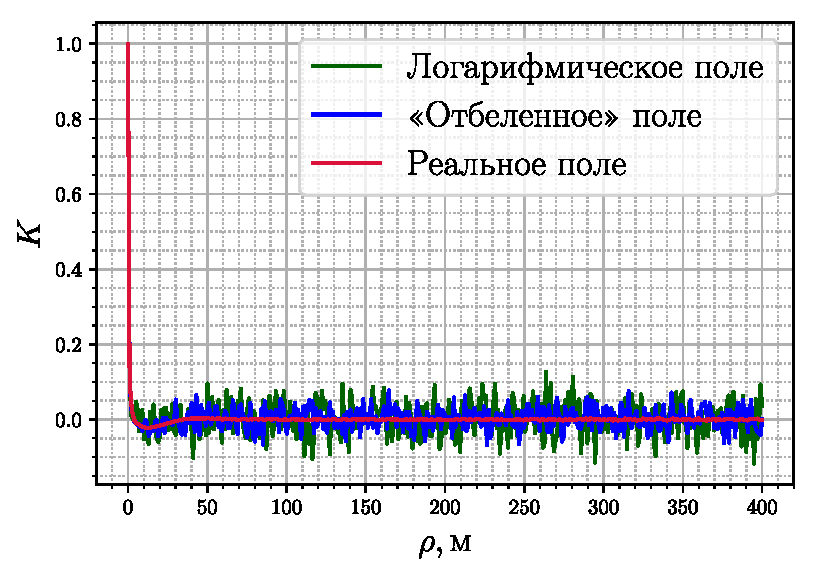
\includegraphics[width=0.6\linewidth]{fig/correlation_angles_wa.pdf}
    \caption{ Нормированная корреляционная функция уклонов для логарифмического расположения
    гармоник (зеленая кривая) и расположения по методу отбеливания спектра
(синяя кривая) для скорости ветра 10 м/с}
    \label{fig:nodes}
\end{figure}

\begin{figure}[h!]
    \centering
    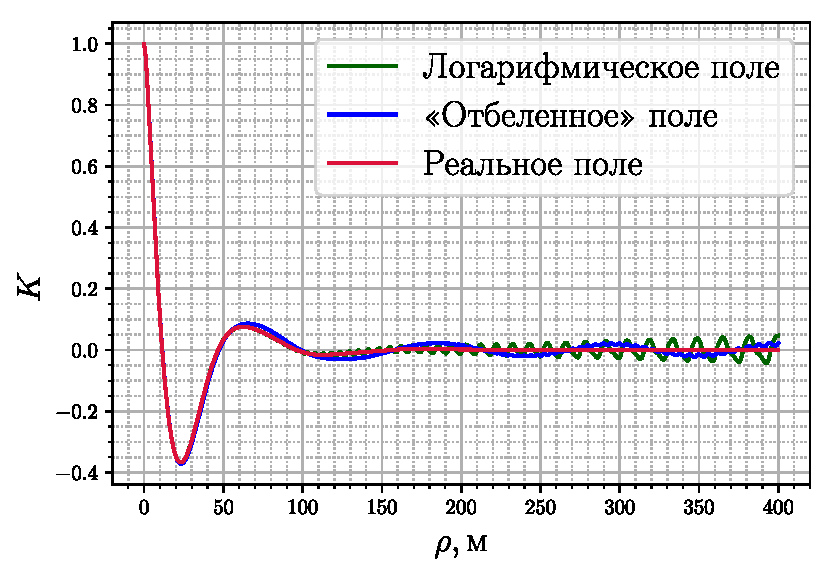
\includegraphics[width=0.6\linewidth]{fig/correlation_height_wa.pdf}
    \caption{ Нормированная корреляционная функция высот для логарифмического расположения
    гармоник (зеленая кривая) и расположения по методу отбеливания спектра
(синяя кривая) для скорости ветра 10 м/с}
    \label{fig:nodes1}
\end{figure}




\begin{figure}[h!]
    \centering
    \begin{subfigure}{0.49\linewidth}
        \centering
        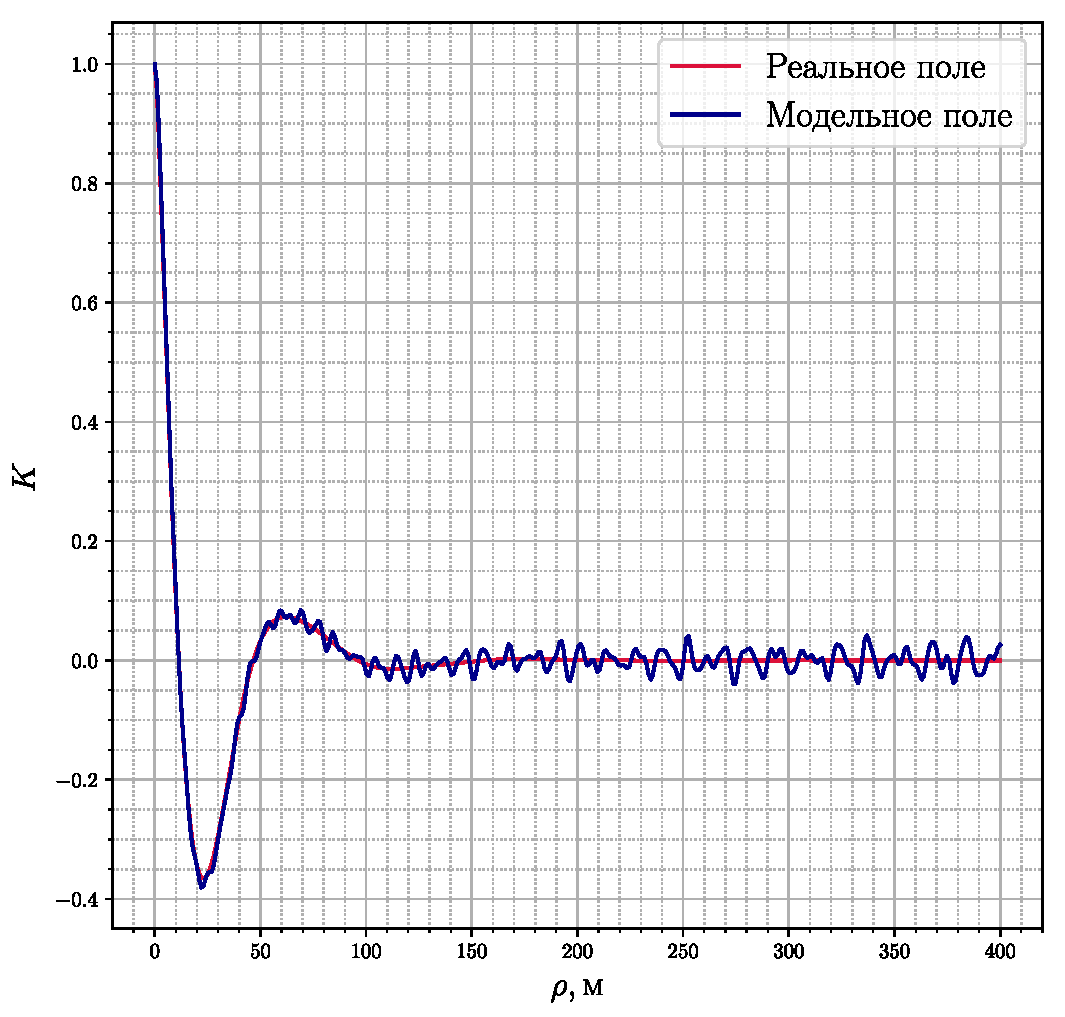
\includegraphics[width=\linewidth]{fig/correlation_height_height2.pdf}
        \caption{}
    \end{subfigure}
    \begin{subfigure}{0.49\linewidth}
        \centering
        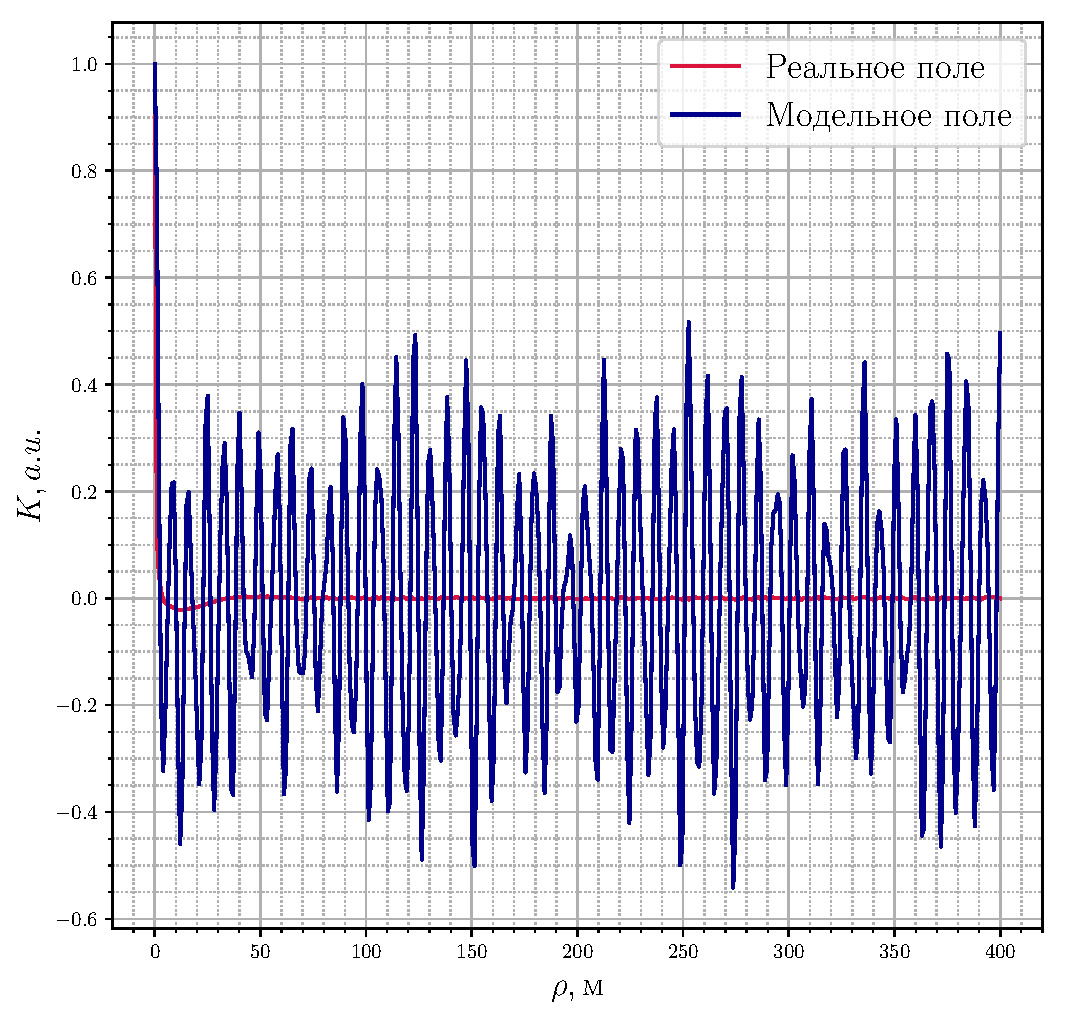
\includegraphics[width=\linewidth]{fig/correlation_angles_height2.pdf}
        \caption{}
    \end{subfigure}
    \caption{ Нормированные корреляционные функции высот (a) и уклонов (b) при расположении гармоник
    по методу <<отбеливания>> спектра по формуле \eqref{eq:ki} }
    \label{fig:ki}
\end{figure}

\begin{figure}[h!]
    \centering
    \begin{subfigure}{0.49\linewidth}
        \centering
        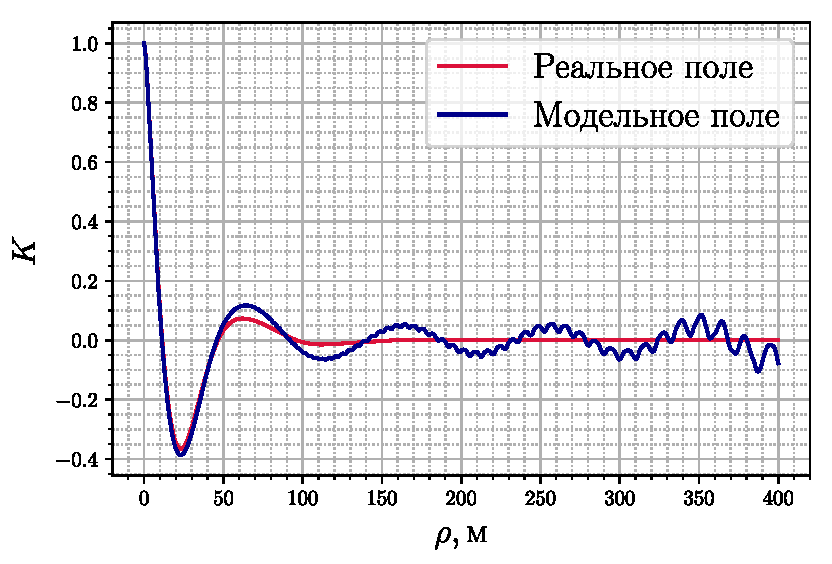
\includegraphics[width=\linewidth]{fig/correlation_height_slopes2.pdf}
        \caption{}
    \end{subfigure}
    \begin{subfigure}{0.49\linewidth}
        \centering
        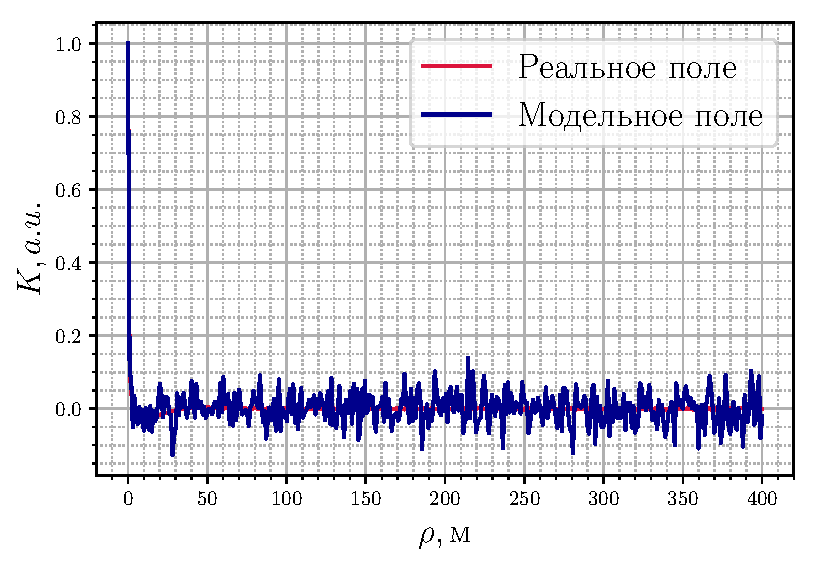
\includegraphics[width=\linewidth]{fig/correlation_angles_slopes2.pdf}
        \caption{}
    \end{subfigure}
    \caption{Нормированные корреляционные функции высот (a) и уклонов (b) при расположении гармоник
    по методу <<отбеливания>> спектра по формуле \eqref{eq:ki_slopes} }
    \label{fig:ki_slopes}
\end{figure}

Из рис. \ref{fig:ki} и \ref{fig:ki_slopes} видно, что определение положения
гармоник по методу отбеливания является эффективным только для той переменной,
которая использовалась в процедуре отбеливания. Для другой переменной результат
получается не слишком хорошим, что свидетельствует о необходимости
использования другого подхода при необходимости одновременного моделирования
поля высот и поля уклонов.

Для решения задачи рассеяния электромагнитного излучения морской поверхностью, 
необходимо моделировать поле высот (определяет форму импульса) и поле уклонов,
которое определяет условие обратного рассеяния падающего изулучения.

\subsubsection{Метод <<отбеливания>> спектра для двух переменных}%
Для такой задачи необходима рассмотреть другую функцию
относительных шумов $Q$, например
\begin{equation}
    \label{eq:Q_modif}
    Q = \frac{\qty(\sigma^{\text{н}}_{\text{шум}})^2}{(\tK^\text{н}(0))^2}+
        \frac{\qty(\sigma^{\text{в}}_{\text{шум}})^2}{(\tK^\text{в}(0))^2},
\end{equation}
где индексы <<н>> и <<в>> соответствуют наклонам и высотам. Учитывая то, что
оба слагаемых в уравнении \eqref{eq:Q_modif} вещественны и положительны, то 
экстремум функции $Q$ можно найти, зная экстремум каждого слагаемого по отдельности. 


Тогда, гармоники, определяющие минимум первого слагаемого описываются
формулой \eqref{eq:ki}, а минимум второго -- формулой \eqref{eq:ki_slopes}.  
На рис. \ref{fig:13} представлено расположение гармоник по методу
<<отбеливания>> спектра для высот и наклонов. Число гармоник было взято
небольшим (N=32), чтобы лучше было заметно распределение, получаемое при
применении метода. Поскольку получившиеся распределения имеют мало общих
корней, то сложно написать одну функцию распределения гармоник, которая будет
удовлетворять и минимуму шума высот и минимуму шума уклонов. Поэтому
предлагается в дальнейшим объединять обе функции распределения. Подобное
совмещенное расположение гармоник представлено на рис. \ref{fig:14}, где синим
цветом обозначены 128 гармоник, расположенные по формуле для отбеливания
спектра высот \eqref{eq:ki}, а красным цветом обозначены 128 гармоник, расположенных по формуле
для отбеливания спектра уклонов \eqref{eq:ki_slopes}.

\begin{figure}[H]
    \begin{subfigure}{0.49\linewidth}
        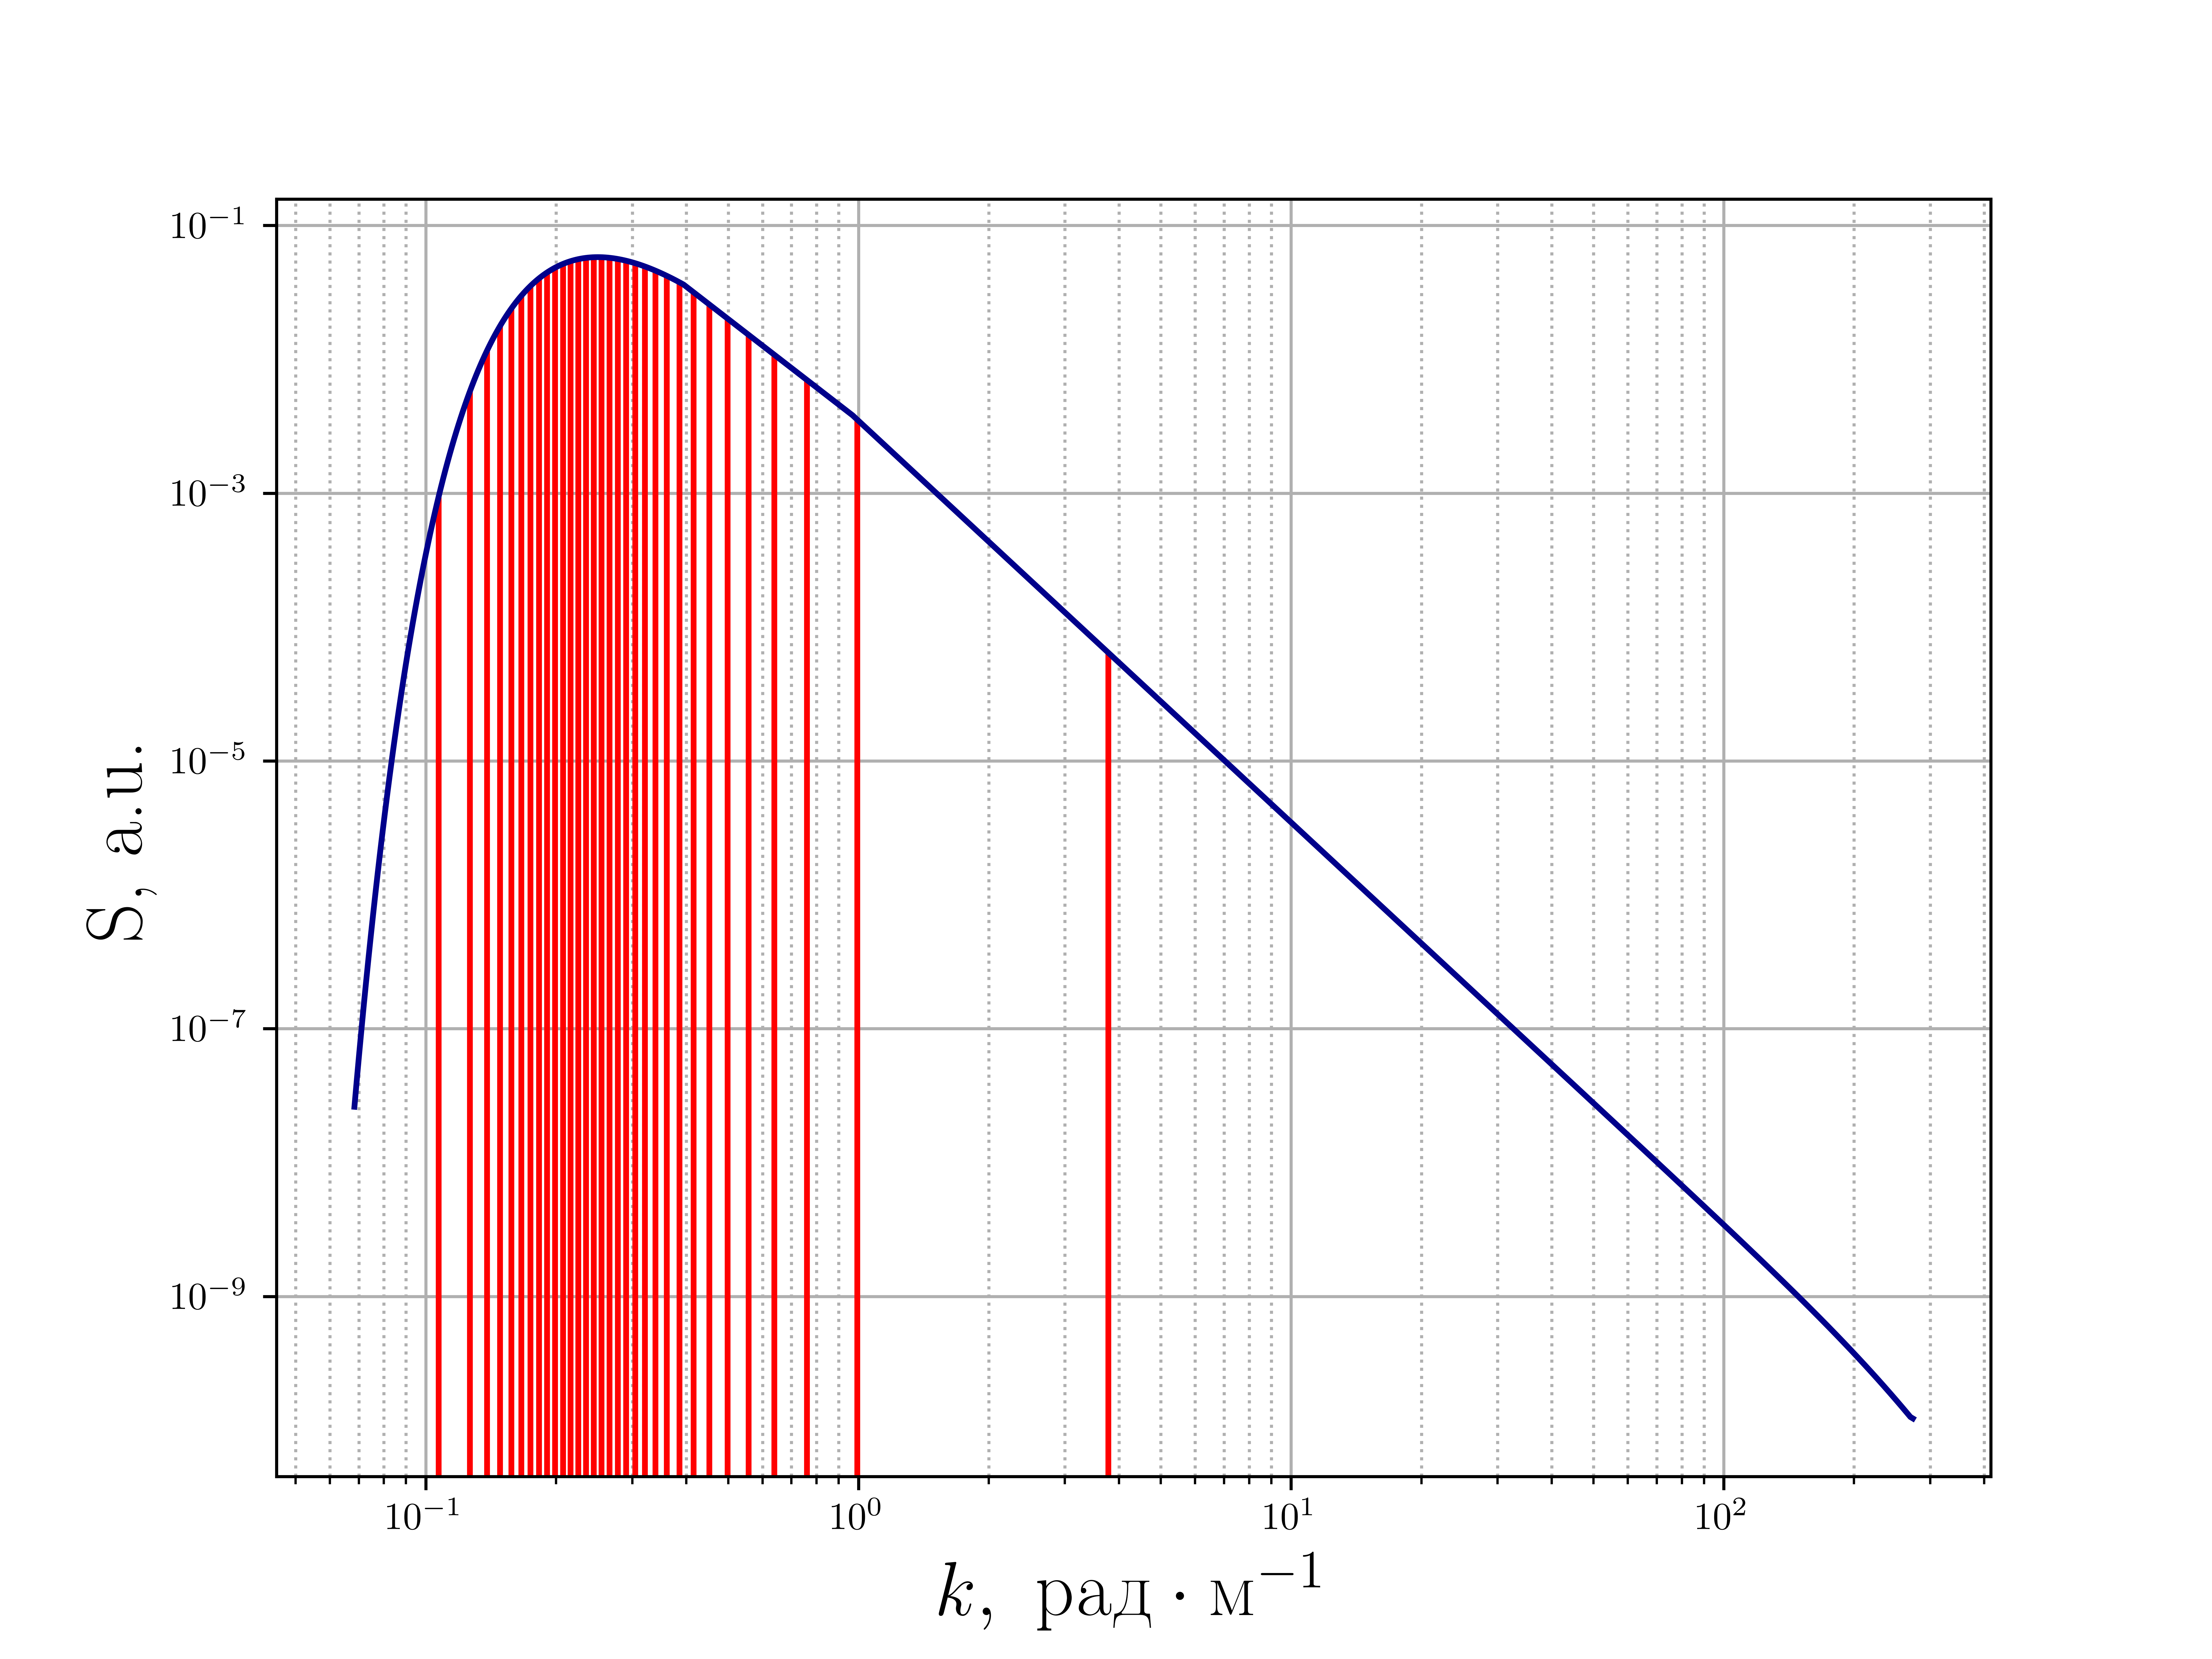
\includegraphics[width=\linewidth]{fig/fig1}
        \caption{}
    \end{subfigure}
    \begin{subfigure}{0.49\linewidth}
        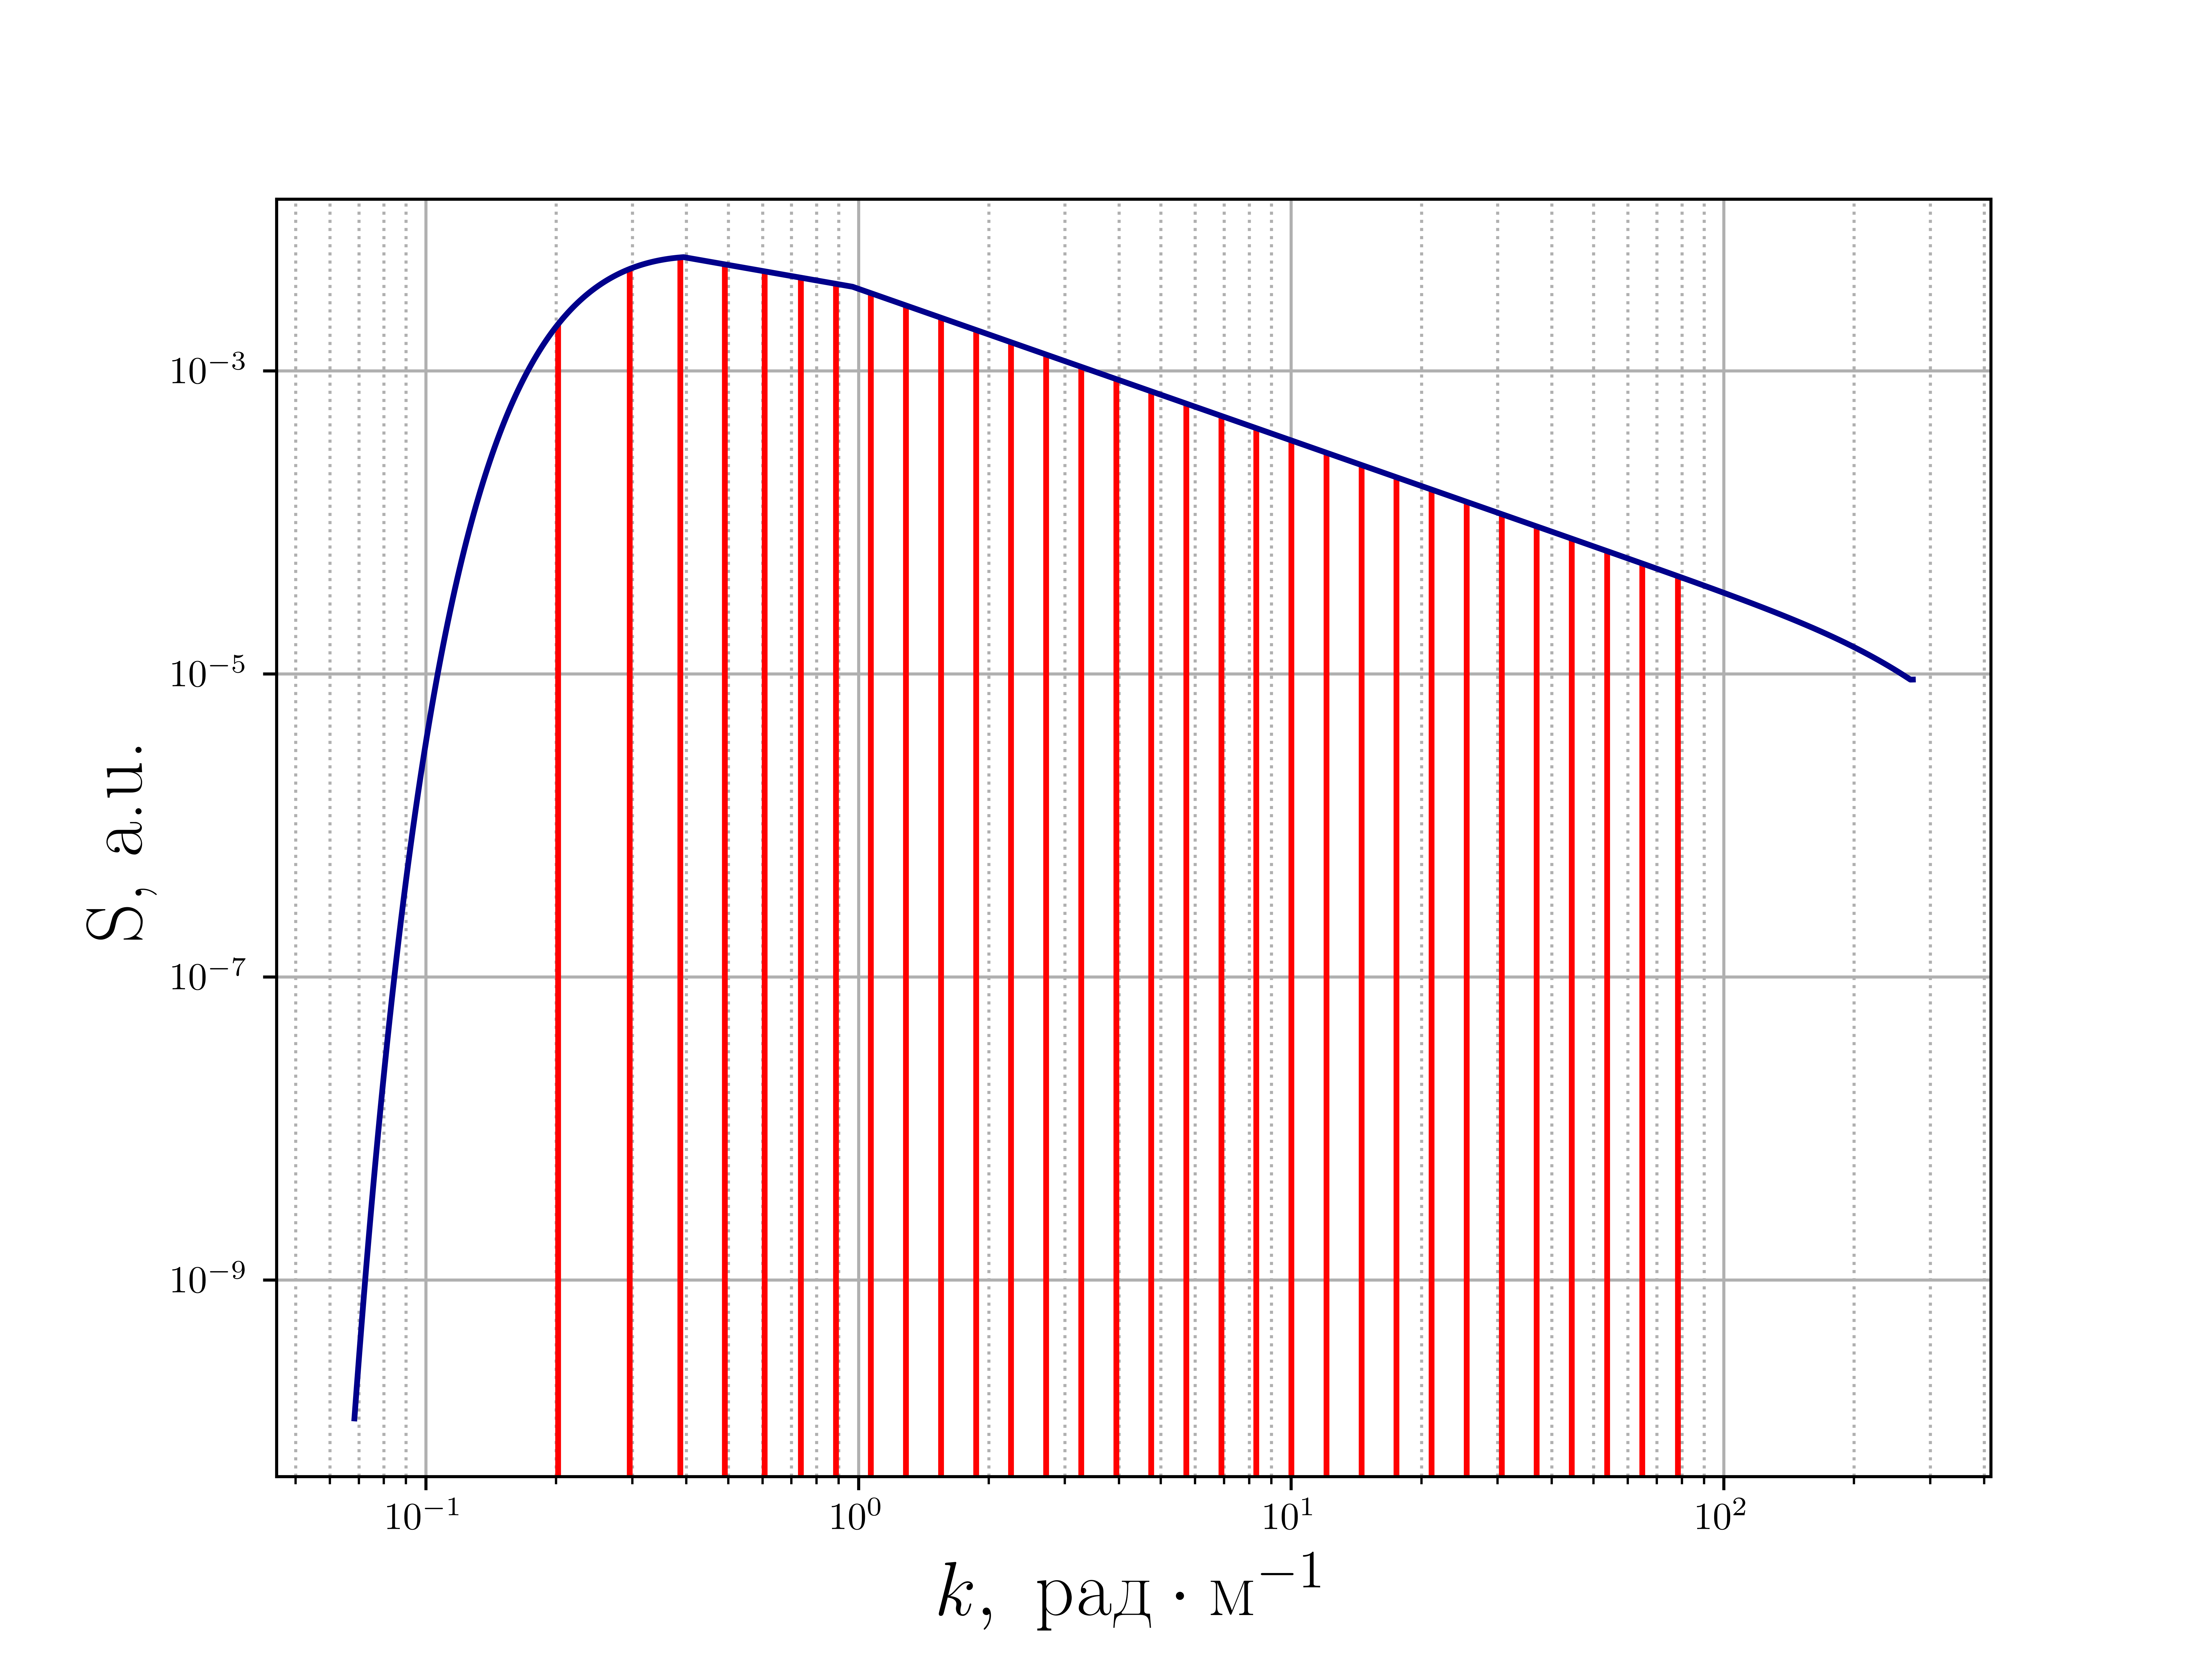
\includegraphics[width=\linewidth]{fig/fig2}
        \caption{}
    \end{subfigure}
    \caption{Расположение гармоник для отбеливания (a) высот, (b) уклонов}
    \label{fig:13}
\end{figure}

\begin{figure}[H]
    \begin{subfigure}{0.49\linewidth}
        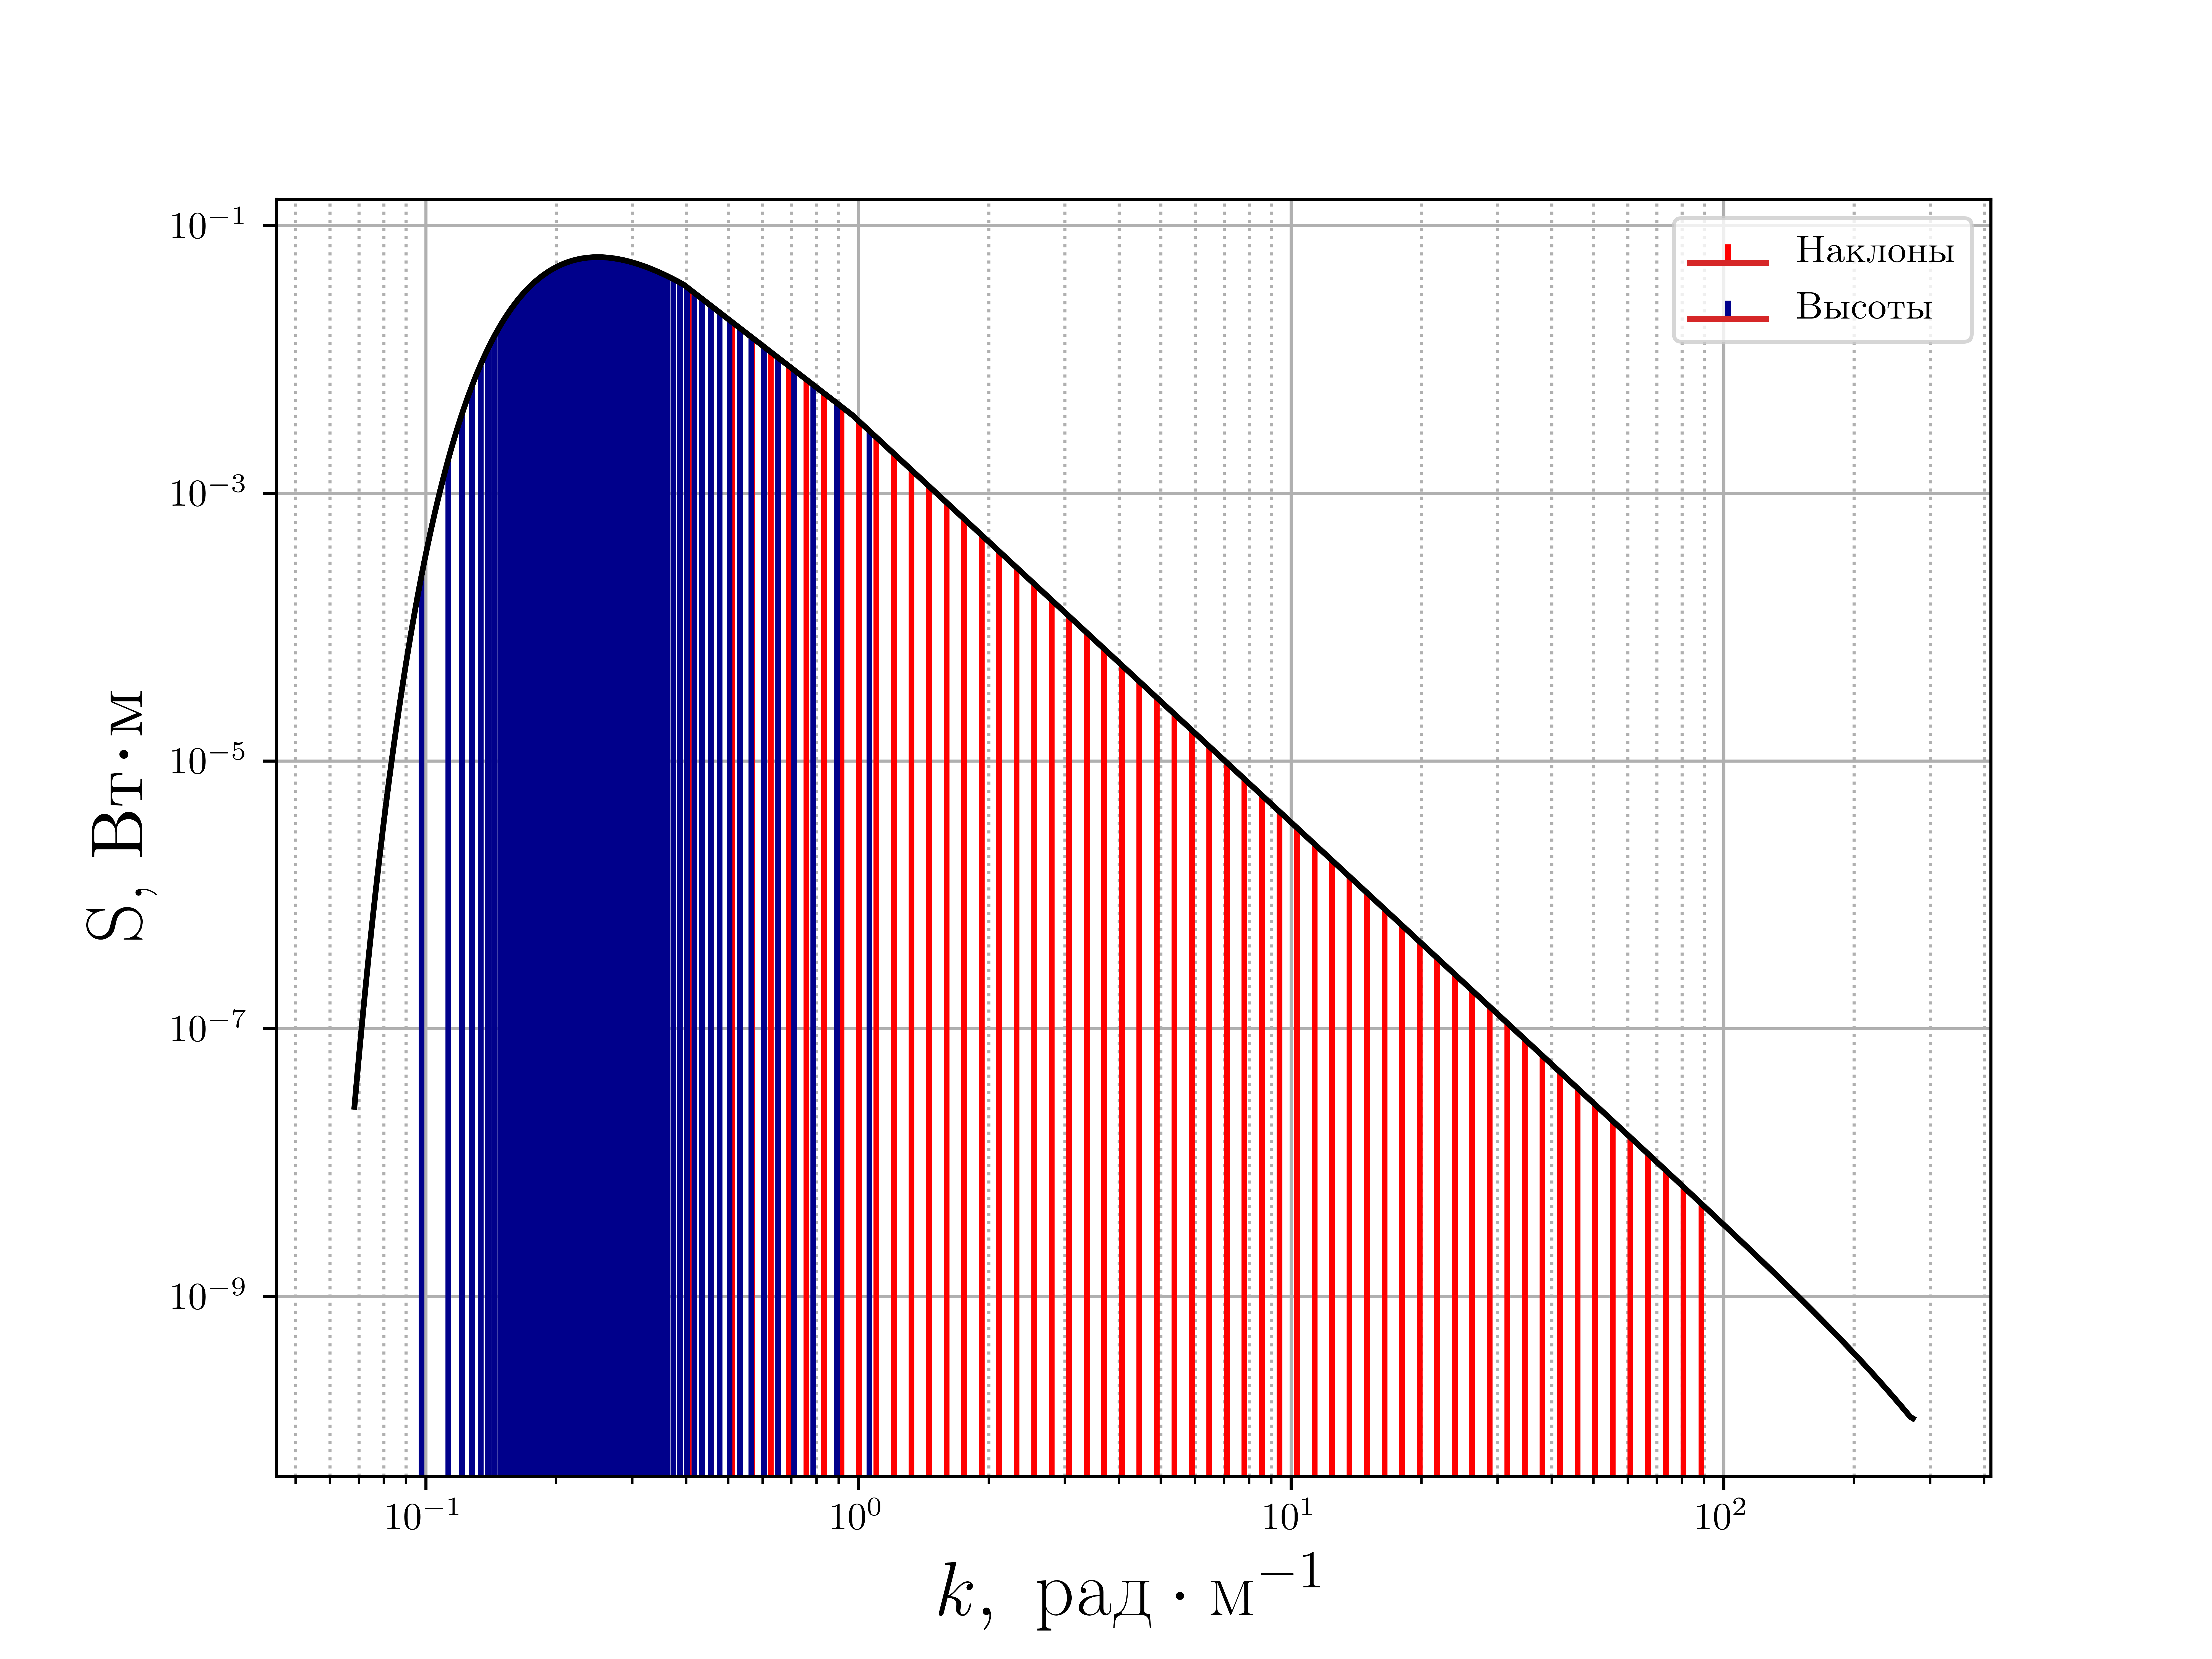
\includegraphics[width=\linewidth]{fig/fig3}
        \caption{Совмещенное расположение гармоник для отбеливания}
    \end{subfigure}
    \begin{subfigure}{0.49\linewidth}
        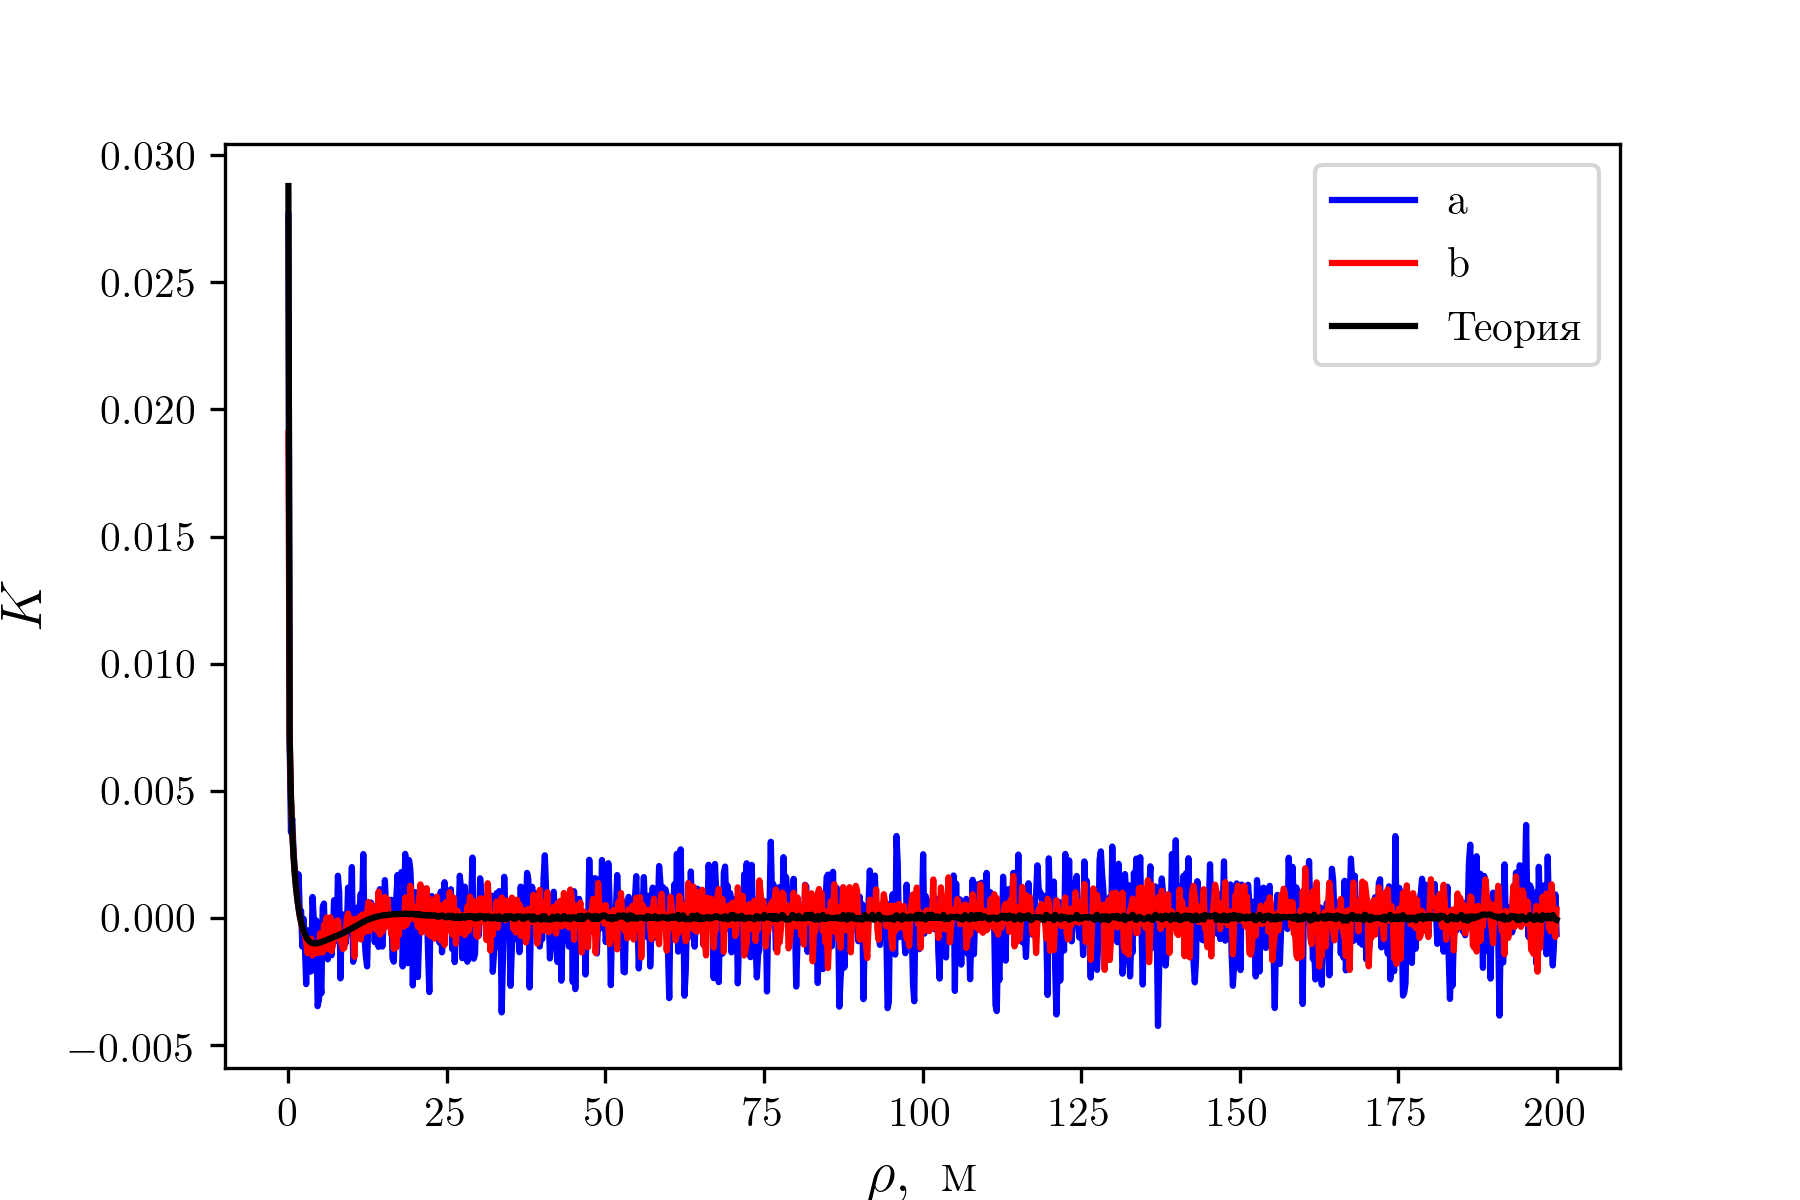
\includegraphics[width=\linewidth]{fig/water/whitening}
        \caption{Корреляционная функция наклонов для различного расположения
        гармоник в частотной области: (a) логарифмическое распределение, (b)
    метод <<отбеливания>> спектра}
    \end{subfigure}
    \caption{}
    \label{fig:14}
\end{figure}

Таким образом, двумерный вариант метода отбеливания является эффективным
способом выбора расположения гармоник для численного моделирования морской
поверхности, задаваемой моделью спектра.


\subsubsection{Аппаратное ускорение моделирования}%
\label{ssub:apparatnoe_uskorenie_modelirovaniia}


В прошлом разделе мы обсуждали как можно ускорить без потери качества процесс моделирования за счет уменьшения количества гармоник в спектре волнения.

Когда с математической точки зрения все оптимизировано можно перейти к
программной оптимизации: поскольку основное время моделирования приходится на
суммирование в цикле по формуле \eqref{eq:surface2d} , на который приходится
$N\times M \times X \times Y$ итераций, где $N$ – число гармоник в частотном
спектре, $M$ – число гармоник в азимутальном распределении, X – размер сетки
вдоль оси $x$, $Y$ – размер сетки вдоль оси $y$. Этот цикл требует больших
затрат мощности и времени и именно его мы можем значительно ускорить благодаря
его внутренней простоте.

Современные центральные процессоры (CPU) уже давно имеют в своём распоряжении
несколько (обычно 4-8) вычислительных ядер, которые в нередко в несколько
потоков могут производить вычисления.

Самое очевидное, что можно сделать – это выполнять програмный код не в одном потоке процессора, а специальным образом разделить координатную сетку на блоки и вычислять каждый блок в отдельном потоке.

Но ещё быстрее можно произвести вычисления на графическом процессоре (GPU).
Современные GPU имеют порядка 1000 вычислительных ядер, что позволяет очень
сильно ускорить процесс моделирования за счет распараллеливания вычислений
между ядрами.

На рисунке рис. \ref{fig:gpucpu} приведено сравнение многопоточных вычислений на CPU и GPU из
одной ценовой категории. Поверхность моделировалась при $N=2048$, $M=512$. При
вычислении поверхности $256\times256$ точек центральному процессору для этого
требуется 2030 секунд, в то время как графический процессор справится с этой
задачей лишь за 71 секунду.

\begin{figure}[H]
    \centering
    \begin{subfigure}{0.49\linewidth}
        \centering
        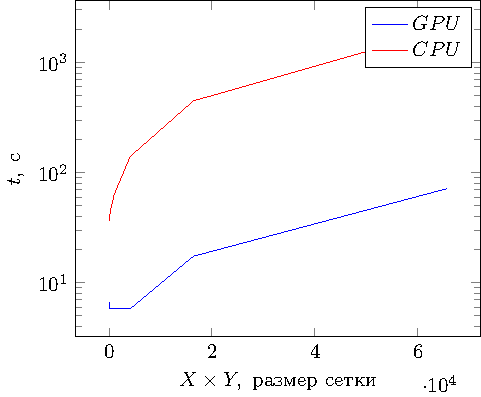
\includegraphics[]{fig/water/gpucpu.pdf}
    \end{subfigure}
    \begin{subfigure}{0.49\linewidth}
        \centering
        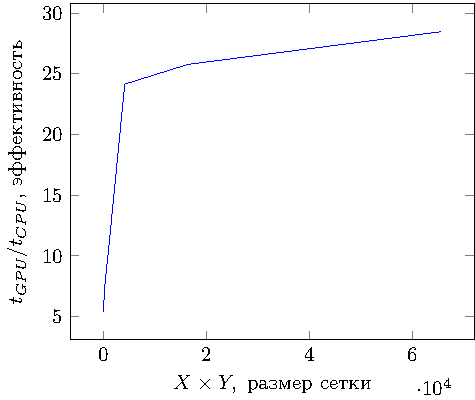
\includegraphics[]{fig/water/gpucpu1.pdf}
    \end{subfigure}
    \caption{Сравнение времени моделирования двумерной поверхности на CPU и
    GPU: (a) время вычисления поверхности на сетке размером $X \times Y$;
(b) относительная скорость вычислений $t_{GPU}/t_{CPU}$;}
    \label{fig:gpucpu}
\end{figure}

Программную реализацию вычислений на графическом процессоре можно посмотреть в
приложении \ref{sec:code} в листинге \ref{lst:kernel}.

\subsection{Заостренная морская поверхность}
\label{sub:cwm}

Как отмечалось ранее, при моделировании морской поверхности синусоидами мы
получаем нулевое среднее значение высот, что не позволяет смоделировать
поправки на состояние морской поверхности. 

Ниже предлагается модель поверхности у которой средний уровень не равен нулю.



\subsubsection{Двумерный случай}%
\label{ssub:odnomernyi_sluchai}

Рассмотрим для начала задачу моделирования двумерной поверхности суммой гармоник с детерменированными амплитудами и случайными фазами
 \begin{equation}
     z = \sum\limits_{j=0}^{N} A_j \cos(k_j x + \psi_j)
 \end{equation}

Чтобы получить модель заостренной волны введем нелинейное преобразование координат
\begin{equation}
    \qty{x,z(x)} \longrightarrow \qty{x + D(x),z(x)},
\end{equation}
где $D(x)$ горизонтальное смещение
\begin{equation}
    D(x) =  \frac{i}{2\pi} \int\limits_{-\infty}^{\infty}   \hat z e^{ikx} \dd{k},
\end{equation}
а $S(k)$ -- прямое Фурье преобразование исходной поверхности
\begin{equation}
    S(k) = \int\limits_{-\infty}^{\infty} z(x) e^{-ikx} \dd x 
\end{equation}

В нашем случае, функция $D(x)$ примет вид: 
\begin{equation}
    \begin{cases}
    x = x_{0} \underbrace{
    - \sum\limits_{j=0}^{N} A_j \sin(k_j x_0 + \psi_j)
    }_{D(x)} \\
    z = \sum\limits_{j=0}^{N} A_j \cos(k_j x_{0} + \psi_j)
    \end{cases}
\end{equation}

Иными словами мы будем моделировать волнение не суммой гармонических функций, а 
суммой трохоид. 

Для того, чтобы наше преобразование $D(x)$ имело физический смысл
необходимо, чтобы для каждой $j$-ой гармоники выполнялось соотношение 
\begin{equation}
    A_j k_j \ll 1 
\end{equation}

\paragraph{Статистические моменты}%

Запишем характеристическую функцию нового случайного процесса $z(x_0(x))$ по
определению
 \begin{equation}
    \label{eq:Phi1}
    \Theta(i\theta) = \mean{ e^{i \theta z(x_0(x))}}
\end{equation}
Поскольку процесс $z(x_0)$ стационарный, то от \eqref{eq:Phi1} можно перейти к
\begin{equation}
    \label{eq:Phi2}
    \Theta(i\theta) = \lim_{L \to \infty} \frac{1}{2L} \int\limits_{-L}^{L} e^{i \theta z(x_0)
    }\dd x = 
    \lim_{L \to \infty} \frac{1}{2L} \int\limits_{-L}^{L} e^{i \theta z(x_0)} \qty( 1 + D'(x_0) ) \dd x_0
\end{equation}

Поскольку $z(x_0)$ стационарный процесс, а  $D'(x_0)$ стационарен по нашему
определению, то  \eqref{eq:Phi2} преобразуется к виду
\begin{equation}
    \label{eq:Phi}
    \Theta(i\theta) = (1 - i \theta \sigma_1^2) 
    \exp(-\frac{1}{2} \theta^2 \sigma_0^2),
\end{equation}
где $\sigma^2_n = \int\limits_{-\infty}^{\infty}  k^n S(k) \dd k$ -- момент
$n$-го порядка спектра волнения.

Зная характеристическую функцию не сложно получить необходимые статистические
моменты дифференцируя \eqref{eq:Phi}
\begin{equation}
    m_n = i^{-n} \dv[n]{\Theta(i\theta)}{\theta} \eval_{\theta = 0}
\end{equation}

Следовательно, среднее и дисперсия случайного процесса $z(x_0)$ будут
равны
\begin{gather}
    \mean{z} = - \sigma_1^2, \quad \mean{z^2} = \sigma_0^2 \\
    \mean{z^2} - \mean{z}^2 = \sigma_0^2 - \sigma_1^4
\end{gather}

Также не сложно получить связь уклонов в смещенных координатах $x$ с наклонами
в несмещенных координатах $x_0$ пользуясь определением уклонов
 \begin{equation}
    z'(x) = \dv{z(x)}{x} = \frac{z'(x_0)}{1 + D'(x_0)}
\end{equation}



\subsubsection{Трехмерный случай}%

Для трехмерного случая Пирсон \cite{pierson} представил решение
линеаризованных уравнений движения для невязкой жидкости в лагранжевых
координатах. Он показал, что в глубокой воде положение частиц на свободной поверхности задается следующими параметрическими уравнениями
\begin{equation}
    \begin{cases}
        \label{eq:surface2dcwm}
        z(\vec r,t) = \sum\limits_{n=1}^{N} \sum\limits_{m=1}^{M}
        A_n(\kappa_n) \cdot
        F_m(\kappa_n,\phi_m) \cos \qty(\omega_n t + \vec \kappa_n \vec r_0 +
        \psi_{nm}),    \\
        x = x_0 - \sum\limits_{n=1}^{N} \sum\limits_{m=1}^{M}
        A_n(\kappa_n) \cdot
        F_m(\kappa_n,\phi_m) \cos\phi_m \sin\qty(\omega_n t + \vec \kappa_n \vec r_0 +
        \psi_{nm}),\\
        y = y_{0} - \sum\limits_{n=1}^{N} \sum\limits_{m=1}^{M}
        A_n(\kappa_n) \cdot
        F_m(\kappa_n,\phi_m) \sin \phi_m \sin \qty(\omega_n t + \vec \kappa_n \vec
        r_0 + \psi_{nm}),
    \end{cases}
\end{equation}
где $\vec \kappa$ -- двумерный волновой вектор,  
$\vec r_0 = (x_0, y_0)$, $\vec r = (x, y)$


\paragraph{Статистические моменты}
\label{par:statisticheskie_momenty}
В трехмерном случае вычисления аналогичны двумерному случаю, но более
громоздкие.

Введем смешанный $\sigma_{\alpha \beta \gamma}^2$ и начальный $\sigma_n^2$
моменты спектра волнения \cite{nouguier}
\begin{equation}
    \sigma^2_{\alpha \beta \gamma} =  \int\limits_{} \frac{\kappa_x^\alpha
    \kappa_y^\beta}{\kappa^{\gamma}} S(\vec \kappa) \dd \vec \kappa,\quad
    \sigma_n^2 = \int\limits_{}^{} \kappa^n S(\vec \kappa) \dd \vec \kappa 
\end{equation}
можно получить следующую характеристическую функцию для трехмерного волнения
\begin{equation}
    \label{eq:char}
    \Phi(\theta) = (1 - i \theta \sigma_1^2 + \theta^2 \Sigma_1)
    \exp(-\frac{1}{2} \theta^2 \sigma_0^2),
\end{equation}
где $\Sigma_1 = \sigma^4_{111} - \sigma_{201}^2 \sigma_{021}^2$.

Из этой характеристической функции можно получить необходимые моменты процесса
\begin{equation}
    \mean{z} = - \sigma_1^2, \quad \mean{z^2} = \sigma_0^2 - 2 \Sigma_1
\end{equation}
 
На рис. \ref{fig:pdf}b представлены срезы трехмерной морской поверхности 
для стандартного подхода и метода заостренной волны. На рис. \ref{fig:pdf}a
изображена теоретическая плотность вероятности наклонов для двух подходов. 

 \begin{figure}[h!]
    \centering
     \begin{subfigure}{0.49\linewidth}
        \centering
        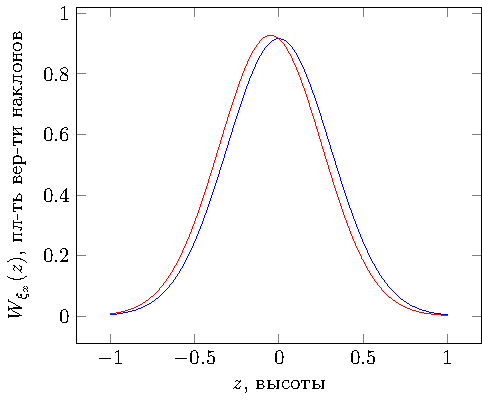
\includegraphics[]{fig/water/pdf_cwm}
        \caption{}
    \end{subfigure}
    \hfill
     \begin{subfigure}{0.49\linewidth}
        \centering
        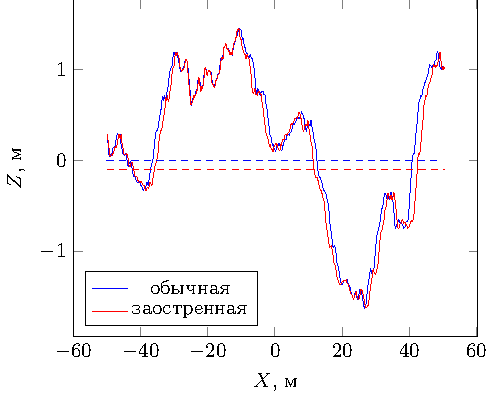
\includegraphics[]{fig/water/surface_cwm.pdf}
        \caption{}
    \end{subfigure}
    \caption{(a) Плотность вероятности уклонов $W_{\xi_x}(z)$ для линейной
        поверхности (синяя кривая) и заостренной поверхности (красная кривая) в
        зависимости от высот $z$ при скорости ветра 10 м/с \\
    (b) Срез поля высот морской поверхности для стандартного подхода (синяя
кривая) и модели заостренной поверхности (красная кривая) при скорости ветра 10
м/с. Пунктиром показан средний уровень соответствующей поверхности}
    \label{fig:pdf}
\end{figure}
На рис. \ref{fig:evolution} представлена эволюция во времени гребня волны для
двух методов. 

\begin{figure}[H]
    \centering
    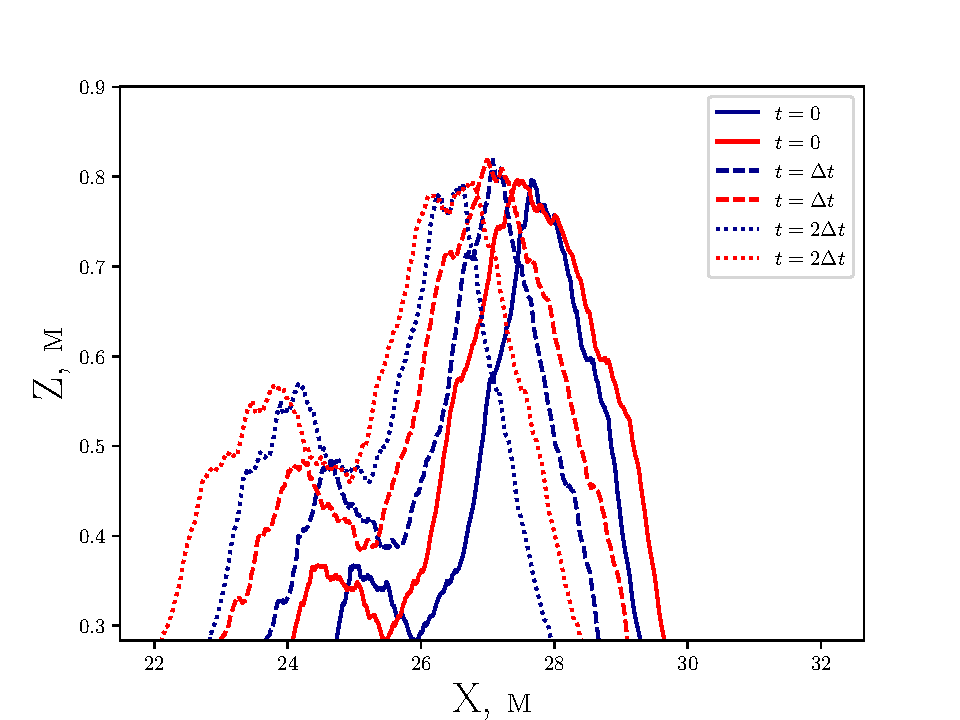
\includegraphics[width=0.8\linewidth]{fig/evolution}
    \caption{Эволюция поверхности, построенной стандартным подходом в сравнении
    с моделью заостренной поверхности}
    \label{fig:evolution}
\end{figure}



На практике средний уровень морской поверхности не совпадает с тем, что может
определить альтиметр. Этот эффект возникает из-за того, что площадь впадин на
поверхности превышает площадь гребней, а значит во впадинах будет больше
отражающих зеркальных точек. 
Из вида характеристической функции $\Phi(\theta)$ в формуле  \eqref{eq:char} мы
можем найти связь плотности вероятности наклонов обычной поверхности с
заостренной
\begin{equation}
    \tilde P_{\xi_x}(z) = 
    P_{\xi_x}(z)\qty(1 + 
                    \frac{\Sigma_1}{\sigma_0^2} -
                    \frac{\sigma_1^2}{\sigma_0^2} z -
                    \frac{\Sigma_1}{\sigma_0^4}z^2), 
\end{equation}
где $P_\xi(z)$ -- гауссовая плотность вероятности наклонов линейной
поверхности,  $z$ -- высоты морской поверхности.


На рис. \ref{fig:pdf} изображен график функции $\tilde P_{\xi_x}$ в сравнении с
функцией $P_{\xi_x}(z)$. Можно заметить, что область нулевых наклонов, а значит
и отражающих точек функции $\tilde P_{\xi_x}(z)$ смещается в сторону
отрицательных высот, что приводит к изменению длительности импульса отраженного
от такой поверхности импульса. 
Это приводит к изменению формы переднего фронта импульса, излучаемого
радиолокатором. 
%О значении этого эффекта речь пойдет следующих разделах.

